\documentclass{report}

\usepackage[top=2cm, left=2cm, right=2cm, bottom=2cm]{geometry}
\usepackage{amsmath}
\usepackage{amsfonts}
\usepackage{mdframed}
\usepackage{cancel}
\usepackage{wrapfig}
\usepackage{tikz}
\usetikzlibrary{arrows}
\usetikzlibrary{decorations.pathmorphing}
\usetikzlibrary{decorations.pathreplacing}
\usetikzlibrary{patterns}
\usetikzlibrary{shapes}

\newcommand\WLOG{{\small\textbf{WLOG}}}

\title{Production Systems}
\author{Henri LEFEBVRE}
\pagestyle{headings}

\begin{document}
    \hspace{\textwidth}
    \vspace{3cm}
    \begin{center}
        {\Large UNIVERSITA DEGLI STUDI DI GENOVA}
        \rule{\textwidth}{.3mm}\\
        \vspace{.5cm}
        {\huge\bfseries Production Systems }\\
        \vspace{.2cm}
        \rule{\textwidth}{.3mm}\\
        \vspace{1cm}
        {\large Henri Lefebvre}
    \end{center}
    \begin{figure}[h!]\thispagestyle{empty}\end{figure}
    \newpage

    \tableofcontents

    \setlength\parskip{0.5cm}

    \chapter*{Introduction}
    \addcontentsline{toc}{chapter}{Introduction}
    Any system can be regarded as some sort of "black box" or "machine" that turns a certain number of inputs into one or multiple output. Production systems do not escape that definition and can be viewed as a system transforming raw materials into final products. Actually, the inputs are more general and complex than just raw materials, for example, one can consider energy, workforce, decisions and many others as inputs of our system. As well, the outputs are generally not only a final product but also scraps or waste. Scrap corresponds to the portion of raw material that we loose with respect to the technology we utilize for transforming the raw materials into final products. Wastes, on the other hand, are immaterial. The figure (\ref{intro:production-system}) sums up what have been said.

\begin{figure}[h!]
    \centering
    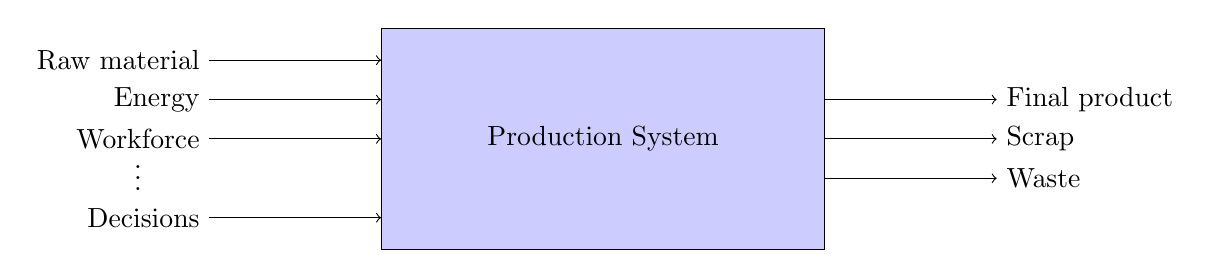
\begin{tikzpicture}
        % system
        \node[draw,fill=blue!20,minimum size=2em, minimum height=8em, minimum width=16em] at (0,0) (box) {Production System};

        % inputs
        \node at (-5, 1) (raw material) [left] {Raw material};
        \node at (-5, .5) (energy) [left] {Energy};
        \node at (-5, 0) (workforce) [left] {Workforce};
        \node at (-5, -1) (decisions) [left] {Decisions};

        % outputs
        \node at (5, .5) (final product) [right] {Final product};
        \node at (5, 0) (scrap) [right] {Scrap};
        \node at (5, -.5) (waste) [right] {Waste};

        % links
        \draw[->] (raw material) -- (raw material-|box.west);
        \draw[->] (energy) -- (energy-|box.west);
        \draw[->] (workforce) -- (workforce-|box.west);
        \draw[->] (decisions) -- (decisions-|box.west);
        \path (workforce) node (decisions) [below] {$\vdots$};

        \draw[<-] (final product) -- (final product-|box.east);
        \draw[<-] (scrap) -- (scrap-|box.east);
        \draw[<-] (waste) -- (waste-|box.east);
    \end{tikzpicture}
    \caption{\label{intro:production-system}General production system}
\end{figure}

The objective of this course is to analyse how we can make our production system more efficient with respect to some criteria (time, money, ...). Of course, our production depends on the methods and on the technolgies we use to manufacture our goods, but these are rather concerns for mechnanical engineers or more specific fields (chemistry, process engineering, ...). Actually, this course focuses on the only input we can, at our level, act uppon, which is : decisions.

To understand how decisions can improve (or worsen) our productivity, let's take a very simple example. Consider the following task : "Drilling four holes in a piece of wood". And let $X$ be the rate of production. Consider as well that the "drilling" operation needs some set-up time in order to prepare the right borer and to turn on the machine. Let's denote by $T_S$ this set-up time and by $T_H$ the operation time which is necessary to actually drill the wooden piece. There are plenty of ways to perform such task, one idea is to drill one hole at a time, stopping the machine after each drill. But this wouldn't be a very clever way since we would have to wait for the set-up time for each hole we want to make. Another idea is to perform a batch of holes in a row so that we only account for the set-up time once for all the batch. The two situations are presented in the GANT diagram in figure (\ref{intro:gant}).

\begin{figure}[h!]
    \centering
    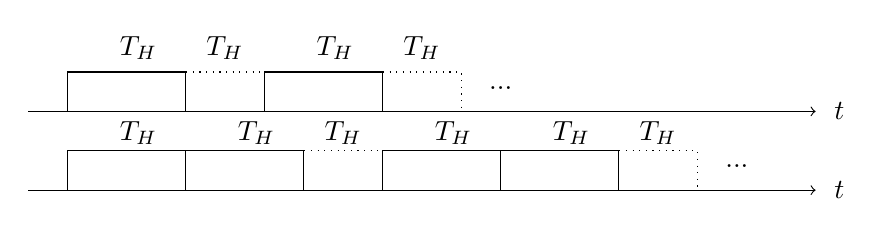
\begin{tikzpicture}
        % first gant
        \draw [->] (0,0) -- (10,0);
        \draw (10.3, 0) node {$t$};

        \draw (.5, 0) rectangle (2, .5);
        \draw (1.4, .8) node {$T_H$};

        \draw [dotted] (2, 0) rectangle (3, .5);
        \draw (2.5, .8) node {$T_H$};

        \draw (3, 0) rectangle (4.5, .5);
        \draw (3.9, .8) node {$T_H$};

        \draw [dotted] (4.5, 0) rectangle (5.5, .5);
        \draw (5, .8) node {$T_H$};

        \draw (6, .3) node {...};

        % second gant
        \draw [->] (0,-1) -- (10,-1);
        \draw (10.3, -1) node {$t$};

        \draw (.5, -1) rectangle (2, -.5);
        \draw (1.4, -.27) node {$T_H$};

        \draw (2, -1) rectangle (3.5, -.5);
        \draw (2.9, -.27) node {$T_H$};

        \draw [dotted] (3.5, -1) rectangle (4.5, -.5);
        \draw (4, -.27) node {$T_H$};

        \draw (4.5, -1) rectangle (6, -.5);
        \draw (5.4, -.27) node {$T_H$};

        \draw (6, -1) rectangle (7.5, -.5);
        \draw (6.9, -.27) node {$T_H$};

        \draw [dotted] (7.5, -1) rectangle (8.5, -.5);
        \draw (8, -.27) node {$T_H$};

        \draw (9, -.7) node {...};
        
    \end{tikzpicture}
    \caption{\label{intro:gant}Two GANT diagrams showing how decisions can influence productivity}
\end{figure}

In the first situation, the rate of production can be expressed as \[ X_1 = \frac{1}{T_H + T_S} \] meaning that we produce one item every $T_H+T_S$ unit of times. For the second situation however, the rate can be computed as \[ X_2 = \frac{2}{2T_H + T_S} = \frac{1}{T_H + \frac{T_S}{2}} \] which means that we produce one item every $T_H+\frac{T_S}{2}$ unit of time, which is smaller. In fact, as long as the batch size increases, the set-up time becomes less and less influent on the production rate since \[ X_k = \frac{k}{kT_H+T_S}\overset{k\rightarrow\infty}{\longrightarrow} \frac{1}{T_H} \] which clearly demonstrates that we can influence our production by making some decisions rather than others. 

The first part of this course will deal with the inventory management in which we'll try to answer to questions like "How and when should we order goods for our production system ?". In fact, we will deal with the different stakeholders to establish good strategies to make our orders. These stakeholders are represented in figure (\ref{intro:agents}). Firstly, the suppliers provides us with some raw materials which can then be stored in a warehouse. When needed, the production system will take some of these materials to transform them into final products. Once done, he will then leave them in another warehouse which will be used to fulfill the demand of such final goods. 

\begin{figure}[h!]
    \centering
    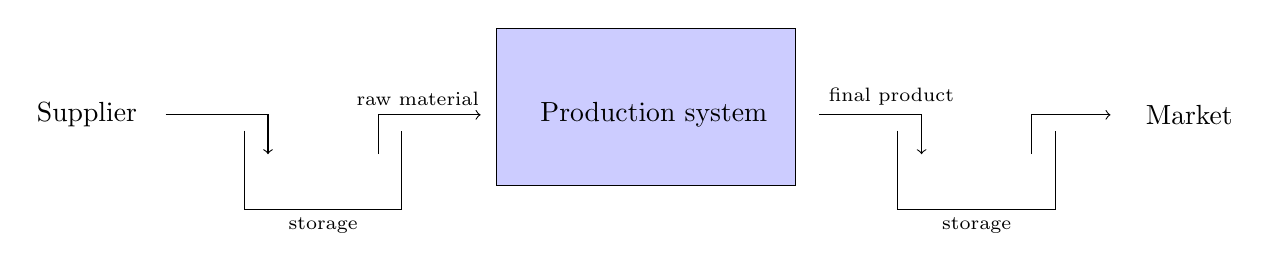
\begin{tikzpicture}
    % supplier -> storage
    \draw (0,0) -- (0,-1) -- (2, -1) -- (2, 0);
    \draw [->] (-1, .2) -| (.3, -.3);
    \draw (-2, .2) node {Supplier};
    \draw (1, -1.2) node {\scriptsize{storage}};

    % storage -> prod sys
    \draw [->] (1.7, -.3) |- (3, .2);
    \draw (1.3, .2) node [above right] {\scriptsize{raw material}};

    % prod sys
    \draw [fill=blue!20] (3.2, -.7) rectangle (7, 1.3);
    \draw (5.2, .2) node {Production system};

    % prod sys -> storage
    \draw [->] (7.3, .2) -| (8.6, -.3);
    \draw (7.3, .2) node [above right] {\scriptsize{final product}};
    
    
    % storage -> market
    \draw (8.3, 0) -- (8.3, -1) -- (10.3, -1) -- (10.3, 0);
    \draw [->] (10, -.3) |- (11, .2);
    \draw (12, .2) node {Market};
    \draw (9.3, -1.2) node {\scriptsize{storage}};

    \end{tikzpicture}
    \caption{\label{intro:agents}Production system agents}
\end{figure}

That being said, it is clear now that any production system aims to fulfill a certain demand taking into account the supply constraints it may encounter. This will be largely discussed futher on.

The figure (\ref{intro:system-types}) depicts the different production system types we can encounter :
\begin{itemize}
    \item Job shops : very specialized entities where, often, solely one product can be produced at the same time. Car repairers are a good example of such production systems. This kind of system is not easily formallized because they are too specific. We will not discuss them in this course. 
    \item Mass production : produces an average number of varieties of goods at average to high rate.
    \item Continuous flow process : produces continuously a given product at very high rate but with very small variety of products.
\end{itemize}

We will focus on both mass production and Continuous flow processes.

\begin{figure}[h!]
    \centering
    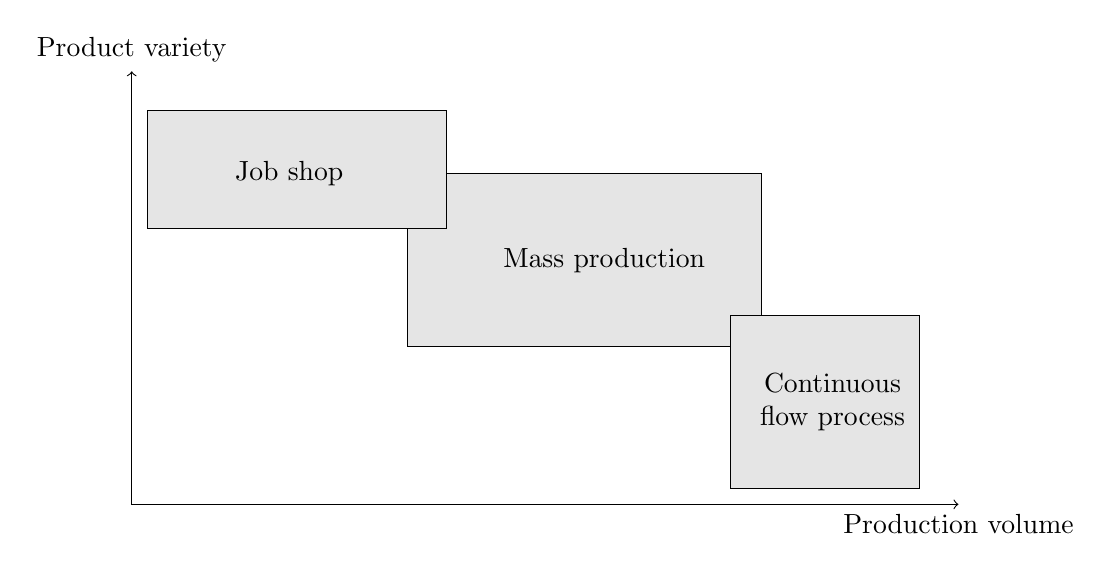
\begin{tikzpicture}
    % axis
    \draw [<->] (0,5.5) node (yaxis) [above] {Product variety} |- (10.5,0) node (xaxis) [below] {Production volume};

    \draw[fill=gray!20] (3.5, 2) rectangle (8, 4.2);
    \draw (6, 3.1) node {Mass production};

    \draw[fill=gray!20] (.2, 3.5) rectangle (4, 5);
    \draw (2, 4.2) node {Job shop};

    \draw[fill=gray!20] (7.6, 0.2) rectangle (10, 2.4);
    \draw [align=center] (8.9, 1.3) node {Continuous \\ flow process};

    \end{tikzpicture}
    \caption{\label{intro:system-types}Production system types}
\end{figure}

The second part of this course will take interest in the bill of materials (which will be further defined) in which we'll look at how to optimize production with respect to the production rate taking into account bottleneck machines in a production site. 

    \part{Inventory management}
    \chapter{Continuous review}
    Inventory management, or storage management, can be qualified as the art of storing and ordering goods in a clever way with respect to some criteria (most often the cost). It can be applied at both the beginning and the end of the production system (even in between actually). At the beginning of this chain, raw materials are delivered by the suppliers and are stored in a warehouse. The storage is emptied when the production site requires some raw materials to be used for production. On the other side of the chain, at the end, the storage is filled with final products and is emptied by the market demand. Though the two situation may appear different in some kind, we can jointly study them considering some sort of "abstract demand" (either production demand or market demand) and some sort of "abstract supplier" (either a real supplier which provides raw material or the production site itself). See figure (\ref{continuous:storage}) for graphical representation.

\begin{figure}[h!]
    \centering
    \begin{tikzpicture}[scale=0.8]
        \draw (-2, .5) node [left] {supplier};
        \draw (7, .5) node [right] {demand};
        \draw (2.5, -3) node [below] {storage};
        \draw (0,0) -| (0,-3) -| (5, 0);
        \draw[->] (-2, .5) -| (.5, -2);
        \draw[<-] (7, .5) -| (4.5, -2);
        \draw [decorate,decoration=snake] (0,-2.3) -- +(5,0);
    \end{tikzpicture}
    \caption{\label{continuous:storage}Storage management parameters}
\end{figure}

To study the inventory management, we introduce models that tend to represent real life cases. Making different assumptions on the demand and supplier, we end with different models. The simplest model is the so called "deterministic model" where all the input data for our problem are supposed to be perfectly known in advance (both the supply and the demand). We will start by studying this model before focusing on a "stochastic model" where the supplier and the demand are modeled by random variables. 

In this chapter, we will study what is called "continuous inventory management". What we mean by this is that the time is modeled by a continuous variable ($t\in\mathbb R$). In the next chapter, we'll deep into "periodic inventory management" where the time is modeled by a discrete variable ($t\in\mathbb N$). 

\section{Deterministic model}

The deterministic model supposes that we exactely know both the demand and the characteristics of our supplier. We denote by $\lambda$ the rate at which the storage is emptied. In the case where our warehouse is at the end of our chain, just after the production site, $\lambda$ represents how many items (final products) we sell by unit of time. If considered at the beginning of the chain, it corresponds to how many items (raw materials) are needed by our production site. This coefficient can be computed as \[ \lambda = \frac{\textrm{nb of items leaving the warehouse}}{\textrm{observed time}} \]

To fullfill that demand, we need to order a certain quantity of good, which will cost us some amount of money. In fact, the costs are of three kinds : 
\begin{itemize}
    \item A \textbf{fixed cost} which we have to pay for each order we make to our supplier. Let $K$ denote this cost, expressed as $euros/order$
    \item An \textbf{inventory cost} which we pay for storing goods in our warehouse, expressed as $euros/(time\times item)$. Let $h$ be the inventory cost.
    \item A \textbf{unitary cost} which corresponds to the price of each item per se. We will refer to this cost as $c$, expressed as $euros/item$
\end{itemize}

For sure, it is easy to see that choosing the right time and quantity to order goods is a matter of balancing between the fixed cost we pay for ordering an independent amount of product and the inventory cost which we pay for storing the goods. If storing products in our warehouse is very expensive for us, we might prefer to order often and pay the fixed cost multiple times rather than paying it just once and be left with a lot of goods we pay a fortune for storing. If, however, the inventory cost is very low (which means that we can store many items for a small amount of money), we'd rather order a lot of products and store them for a long time if needed. So, how do we compute the total cost ? 

Let $T$ be the period of time between the moment we order some goods and the moment our storage goes empty. Note that since the demand is deterministic and known in advance there is no risk of "unpredicted" events which could lead us to be unable to fullill the demand nor to order too many items in such a way that some would remain after some time. Finally, let $Q$ be the number of items we will buy at the beginning of that period. The figure (\ref{continuous:triangles}) sums up some of the introduced variables. 

\begin{figure}[h!]
    \centering
    \begin{tikzpicture}[scale=0.8]
        \draw[<->] (0, 5) node (yaxis) [above] {$I(t)$} |-  (10, 0) node (xaxis) [below] {$t$};

        \draw (.5, 0) -- ++(0, 4) -- ++(3.5, -4) -- ++(0, 4) -- ++(3.5, -4);
        \draw (8, 1) node {...};
        \draw[dotted] (0, 4) node [left] {$Q$} -- (7,4);
        \draw (2.5, 2.5) node {$-\lambda$} ++(3.5, 0) node {$-\lambda$};
        \draw[<->] (.5, -.5) -- (4, -.5);
        \draw (2, -1) node {$T$};

    \end{tikzpicture}
    \caption{\label{continuous:triangles}Inventory level in the deterministic model}
\end{figure}

For a given period of time $T$, we can then compute the total cost as
    \[ J_T = 
        \underbrace{\vphantom{\int}K}_{\textrm{fixed cost}}
        +
        \underbrace{\vphantom{\int}cQ}_{\textrm{price for }Q\textrm{ items}}
        +
        \underbrace{\int_0^T hI(t)dt}_\textrm{storage cost}
    \]
where the integrated part is simply given by $\frac{QT}{2}$ (are of a triangle\footnote{$\int_0^ThIt(t)dt = \int_0^T h\times Q-\lambda t dt = h[Qt-\lambda \frac{t^2}2 ]_0^T = h\frac{2QT-\lambda T^2}{2}$ and since $Q=\lambda T$ we get $\frac{QT}{2}$ by substituting $\lambda$}). 

For sure, we want to minimize the cost for a given period of time. That cost is given by \[ J = \frac{1}{T}\left( K + cQ + \frac{hQT}{2} \right) = \frac{K\lambda}Q + c\lambda + \frac{hQ}{2} \]
Note that we used the fact that $Q = \lambda T$ holds. Regarded as a function of $Q$, we can analyse its variations by derivation (since $Q=0$ does not make any sense for our purpose, it is for sure differentiable) : 
\[
    \begin{cases}
        \frac{dJ}{dQ} &= -\frac{K\lambda}{Q^2} + \frac{h}{2} \\
        \frac{d^2J}{dQ^2} &= \frac{K\lambda}{Q^3}
    \end{cases}
\]

Solving the optimality condition $\frac{dJ}{dQ} = 0$ we get that \[Q^* = \sqrt{ \frac{2K\lambda}{h} } \] can be regarded as a critical point of $J$. And, since the second derivative of $J$ is positive, the value $Q^*$ corresponds to a minimum of our cost function. This quantity is known as the \textbf{Economic Order Quantity} (EOQ) and corresponds to the number of items we should order every $Q/\lambda$ unit of time in order to minimize the total cost. 

We may discuss the obtained formula noting that : (1) if the fixed price for order is very large with respect to the inventory cost, we will by a large amount in once and store it for a long period of time ; (2) if the demand is high, we buy more ; (3) if the inventory cost is large with respect to the fixed cost per order, we will prefer making multiple orders in order to store as less as possible. 

The moment at which we should order that quantity $Q^*$ of goods is given by the characteristics of our supplier. Let $\tau$ be the lead-time of our supplier (difference between the moment we make an order and the moment we actually recieve the products). We define the so called \textbf{reorder point} as $R = \lambda\tau$ which corresponds to the inventory level at which we should call the supplier to make an order\footnote{Note that in the deterministic case, directely using the lead-time is strictly equivalent to using the reorder point, however, three arguments to use the re-order point rather than the lead-time : (1) the reorder point is linked to a quantity that the warehouse can directly control, (2) the deterministic case is a model, which can or can not reflect the reality, using the reorder point assures us that if, for unexpected reasons, we get to the reorder point sooner than planned, we can still make an order at the right time for the new period of time, (3) we will keep using that quantity in the stochastic case.}.

\section{Stochastic model}

In the previous model, we supposed that we could both know perfectly the demand and the lead-time of our supplier. In real life however, such quantities are often subject to variations and are found by estimation. That being said, we can not afford to trust a deterministic formula since we know that life is full of unpredicted and unpredicatable events. Let $x$ be a random variable such that $x\sim\mathcal N(0,1)$. We now model the demand (denoted $d$ by convention in the stochastic model) by a random variable given by $d=\bar d + \sigma_d x$ and the lead-time by $\tau = \bar\tau +\sigma_\tau x$. 

Actually, the stochastic model is a generalisation of the deterministic model and a lot of common aspects will remain true in this model (in the sense that we can derive the deterministic case from the stochastic case). But, since the demand now variates with time, we can no longer rely on an exact formula giving us \emph{exactely} how many goods we have to order in order to have a $0$-inventory-level when we re-order some other goods. Instead, we'd rather save some goods to prevent the fact of being short on stock. That amount of goods is called the \textbf{safety stock} and will be denoted by the variable $s.stock$. Given these informations, what is reasonnable to expect ? 

The expected value of the demand (resp. the leadtime) is $\bar d$ (resp. $\tau$). The reorder point is thus expected to be given by $\bar d\bar\tau$ which, in average, would bring the inventory level to $0$ before re-ordering. To this quantity, we add the safety stock to prevent us from delays of our supplier. \[ R = \bar d\bar \tau + s.stock \] In average, the stochastic model should be exactely the deterministic model shifted up by precisely $s.stock$ goods in the inventory. The figure (\ref{continuous:realisations}) represents two realisations of the demand while figure (\ref{continuous:average}) represents the expected value of our inventory level. 

\begin{figure}[h!]
    \centering
    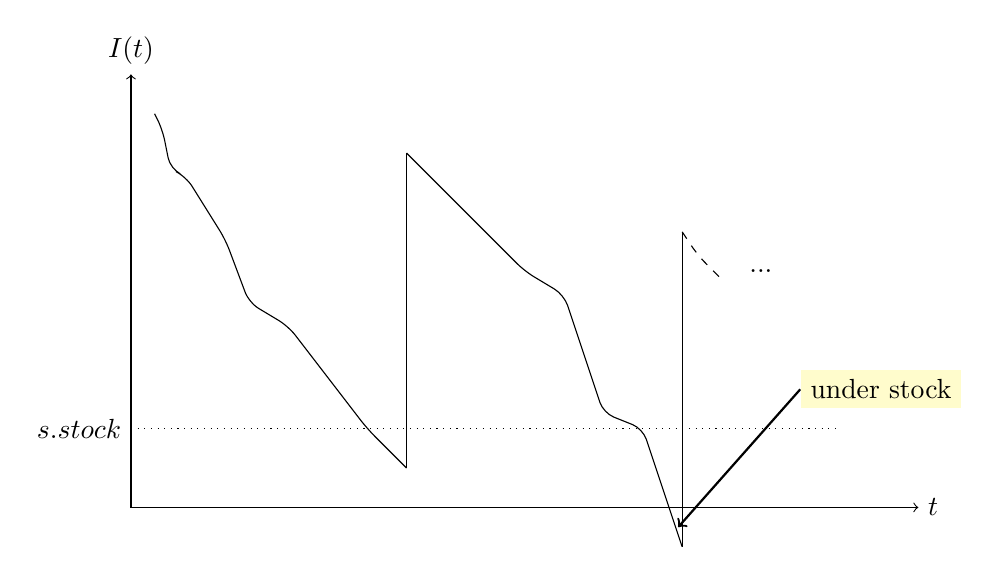
\begin{tikzpicture}
        \draw[<->] (0, 5.5) node [above] {$I(t)$} |- (10, 0) node [right] {$t$};
        \draw[dotted] (0, 1) node [left] {$s.stock$} -- (9, 1);
        \draw[rounded corners] (.3, 5) -- (.4, 4.8) -- (.5, 4.3) -- (.7, 4.2) -- (1.2, 3.4) -- (1.5, 2.6) -- (2, 2.3) -- (3, 1) -- (3.5, .5);
        \draw (3.5, .5) -- (3.5, 4.5);
        \draw[rounded corners] (3.5, 4.5) -- (5, 3) -- (5.5, 2.7) -- (6, 1.2) -- (6.5, 1) -- (7, -.5);
        \draw (7, -.5) -- (7, 3.5);
        \draw[rounded corners, dashed] (7, 3.5) -- (7.2, 3.2) -- (7.5, 2.9);
        \draw (8, 3) node {...};
        \draw[<-, thick] (6.95, -.25) -- (8.5, 1.5) node [right, fill=yellow!20] {under stock};
        
    \end{tikzpicture}
    \caption{\label{continuous:realisations}Two realisations of the demand}
    \begin{tikzpicture}
        \draw[<->] (0, 5.5) node [above] {$\mathbb EI(t)$} |- (10, 0) node [right] {$t$};
        \draw (.3, 1) -- ++(0, 4) -- ++(3.5, -4) -- ++ (0, 4) -- ++(3.5, -4);
        \draw[dotted] (0, 5) node [left] {$Q$} -- (9, 5);
        \draw (2, 3.5) node {$-\bar d$} ++(3.5, 0) node {$-\bar d$};
        \draw[dotted] (0, 1) node [left] {$s.stock$} -- (9, 1);
        \draw (8, 3) node {...};
    \end{tikzpicture}
    \caption{\label{continuous:average}Expected inventory level}
\end{figure}

The expression of the cost must now be updated since we no longer only pay for ordering and storing the goods which are used to fulfill the demand but also for storing some goods as a safety-stock. The total cost is now given by : 

\[ J = \frac{K\bar d}{Q} + c\bar d + \frac{hQ}{2} + h\times s.stock \]

This function of two variables ($Q$ and $s.stock$) is actually well splittable into two functions of one variable denoted by $f(Q)$ and $Q(s.stock)$. It is clear that minimizing the total cost can now be done by minimizing both functions seperately. Regarding the first function $f$, the computations remains the same as in the previous section (deterministic model) and we still have $Q^* = \sqrt{2K\bar d}{h}$. Minimizing $g$ how ever, requires some more analysis. Of course, $g$ is linear with respect to $s.stock$ so the global minimum is $0$ since it cannot be negative. But setting it to $0$ would mean risking to be short on stock at some point. We, somehow, want to control the risks we take and two strategies can be opted for :

\begin{enumerate}
    \item Let $d_\tau$ be the demand over the lead-time $\tau$. It is clear that $d_\tau$ is \emph{linked} to both $d$ and $\tau$ but it is a rather strong assemption to say that these two random variables are \emph{dependent}. Indeed, the realisation of the leadtime of a supplier is not dependent on the global demand\footnote{it is surely linked, for example, during peak demands of a given good, one supplier may have difficulties to satisfy all of his clients, but we cannot consider that a truck getting lost, or breaking down depends on the demand}. $d_\tau$ is thus given by $d_\tau = \bar d_\tau + \sigma_{d_\tau}x $ where $\bar d_\tau = \bar d\bar\tau$ and $\sigma_{d_\tau}=\sqrt{ \sigma_d^2\bar\tau + \sigma_\tau^2\bar d^2 }$. One idea to select effectively the safety stock is to make sure that the probability of being short on stock is lesser than a certain number which we control. Being short on stock is realised when the demand over the lead-time is greater than the reorder point we have choosen. This strategy implies choosing $s.stock$ so that \[ \mathbb P(d_\tau\le R)\ge\alpha = \mathbb P\left(x\le\frac{R-\bar d_\tau}{\sigma_{d_\tau}}\right)\ge\alpha \] where $\alpha$ is called the "fill rate". 
    Using this strategy can be done as follow : 
    \begin{enumerate}
        \item Choose an acceptable probability $\alpha$
        \item Solve the eqution for $X$ and let $\bar X$ be the solution
        \item Subsitute $X$ by $\bar X$ in $s.stock = \bar d_\tau + \sigma_{d_\tau}X$
    \end{enumerate}
    \item As it has been previously said, it holds that we are short on stock when $d_\tau > R$ (more demand during the lead-time than the reorder point). Let $n(R)$ be the average number of unused items (items remaining in the warehouse when we re-order again).  We can compute this quantity with the following formula\footnote{For any random variable $X$ with density function $f$, the average value of $X$ is given by $\int_0^\infty xf(x)dx$} : \[ n(R) = \int_R^\infty (d_\tau-R)f(d_\tau)d(d_\tau) \] However, it is analytically hard to compute. To deal with that problem, we introduce the function $L$ which is called the loss function expressed as \[ L(X) = \int_X^\infty(t-X)f(t)dt\textrm{ where }f\textrm{ is the density of the normal law }\mathcal N(0,1) \] so that \[ n(R) = \sigma_{d_\tau}L(X) \] Finally, by defining the average percentage of unused items with respect to the total number of goods we buy, denoting it by $\beta=\frac{n(R)}{Q^*}$ we can find $s.stock$ so that \[ L(X) = \frac{\beta Q^*}{\sigma_{d_\tau}} \] where $\beta$ should of course be defined \emph{a priori} depending of the market requirements, of course, the lowest $\beta$ is, the greatest is the service.

    Using this second strategy can be done like so :
    \begin{enumerate}
        \item Compute $\sigma_{d_\tau}$
        \item Compute $\frac{\beta Q^*}{\sigma_{d_\tau}}$ and use the table to find the corresponding $X$ denoted $\bar X$
        \item Subsitute $X$ by $\bar X$ in $s.stock = \bar d_\tau + \sigma_{d_\tau}X$
    \end{enumerate}
\end{enumerate}

    \chapter{Periodic review}
    In the previous section, time was supposed to be continuous. In this new chapter however, we will regard time as a discrete variable meaning that we consider fixed size time intervals for our inventory management study. To each of these periods corresponds a certain demand, denoted $d_i$ for period $i$, and a decision (called "action") that we take in order to satisfy the demand, denoted $a_i$. We represent this situation with plots similar to figure (\ref{periodic:plot}) where each box stands for a period of time. The question we have to answer in this chapter is : "What actions do I have to take in order to fulfill the demand minimizing the total cost ?", or similarly : "How many items $a_i$ should I buy in period $i$ to minimize the cost ?"

\begin{figure}[h!]
    \centering
    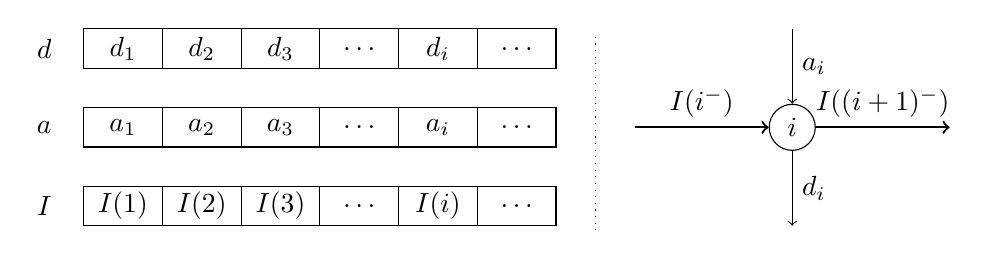
\begin{tikzpicture}
        \draw (.5, .25) node {$d$};
        \foreach \x/\t in {1/$d_1$, 2/$d_2$, 3/$d_3$, 4/$\hdots$, 5/$d_i$, 6/$\hdots$} {
            \draw (\x, 0) rectangle (\x+1, .5);
            \draw (\x+.5, .25) node {\t};
        }

        \draw (.5, -.75) node {$a$};
        \foreach \x/\t in {1/$a_1$, 2/$a_2$, 3/$a_3$, 4/$\hdots$, 5/$a_i$, 6/$\hdots$} {
            \draw (\x, -1) rectangle (\x+1, -.5);
            \draw (\x+.5, -.75) node {\t};
        }

        \draw (.5, -1.75) node {$I$};
        \foreach \x/\t in {1/$I(1)$, 2/$I(2)$, 3/$I(3)$, 4/$\hdots$, 5/$I(i)$, 6/$\hdots$} {
            \draw (\x, -2) rectangle (\x+1, -1.5);
            \draw (\x+.5, -1.75) node {\t};
        }

        \draw[dotted] (7.5, .4) -- ++(0, -2.5);

        \draw (10, -.75) node[circle, draw] (i) {$i$};
        \draw[->, thick] (8, -.75) -- node [above] {$I(i^-)$} (i);
        \draw[->] (10, .5) -- node [right] {$a_i$} (i);
        \draw[->] (i) -- node[right] {$d_i$} (10, -2);
        \draw[->, thick] (i) -- node[above] {$I((i+1)^-)$} (12, -.75);
    \end{tikzpicture}
    \caption{\label{periodic:plot}A representation of the periodic review model}
\end{figure}

With this representation, it becomes clear that, at the end of the $i$-th period, the inventory level, denoted by $I((i+1)^-)$, corresponds to the inventory level we had at the beginning of that period, $I(i^-)$, to which we should add the number of items we have ordered, $a_i$, minus the demand, $d_i$, which corresponds to goods which have been sold out. Hence, \[ I((i+1)^-) = I(i^-) + a_i - d_i \] Thus, by denoting by $h$ the inventory cost and by $K$ the fixed cost per order as we have been doing so far, the total cost can be computed as :
\[
    J = \sum_{i=1}^N\left( K\delta(i) + hI((i+1)^-) \right)
    \textrm{ where }
    \delta(i) = \begin{cases}
        1 &\textrm{ if } a_i > 0\\
        0 &\textrm{ otherwise }
    \end{cases}
\]

Our goal is to minimize this function by choosing relevant $a_i$s. For example, we need to discuss whether it is more profitable to order goods for two periods in a row instead or ordering period per period with respect to the demand. This can be solved by mixed integer linear programming models in an exact way. However, the cost of these methods are not worth it since efficient Heuristics have been developed which are very simple to implement. In this chapter, we will focus on the "Silver-Mill Heuristic". 

Even though it appears clear, note that, if the inventory level in period $0$ is $0$ and if we suppose knowing in advance the exact demand for each period, then it holds that \[ \sum_{i=0}^N a_i \ge \sum_{i=0}^Nd_i \]This can easily be demonstrated by recursivity. Let's suppose that $I_0=0$. Then, and because $I_i\ge 0, \forall i$ in the deterministic model, $I_1=a_1-d_1\ge 0$ which means that $a_1\ge d_1$. So the property is true for the first rank. Let's now suppose, that, for a given rank $k$, we have $\sum^k a_i\ge \sum^k d_i$. Considering $I_{k+1}$, it holds that $I_{k+1} = I_k + a_{k+1} - d_{k+1}$ with $I_k = \sum^k a_i - \sum^k d_i$ so that in definitive $\sum^{k+1}a_i\ge\sum^{k+1}d_i$.

\section{The Wagner-Within Theorem}

The Wagner-Within Theorem tells us about the shape of the solution to our problem. It stipulates that the optimal solution is either that (1) we buy exactely the demand of multiple time periods or (2) we buy exactely the current period demand, but in no case we would buy a fraction of the demand for one time period and buy the rest in another period. The optimal solution cannot be splitted into periods of time. For instance, the optimal solution cannot be to buy 70\% of the forecasted demand of November in September and 30\% of that same demand in October, but rather buy all the corresponding demand for November in September or all the corresponding demand for Novemeber in October. We do not split the orders for one time period. So that, considering $a_1$ for example, we now know that \[ a_1 \in \{ d_1, d_1+d_2, d_1+d_2+d_3, \hdots \} \] In this section we will demonstrate this theorem for the case of two time periods \WLOG. 

Let's consider a time horizon of two periods and, since the demand is supposed to be known in a deterministic way, we can impose that the inventory level at the end of the horizon is zero, $I_2=0$. As well, we'll assume that $I_0$ is zero (no initial inventory level). The inventory level at the end of this time horizon is given by $I_2 = a_1 + a_2 - d_1 - d_2 = 0$ which leads to the equality \begin{equation} a_1 + a_2 = d_1 + d_2 \label{periodic:actions_demand_eq} \end{equation}
In the first time period, we at least have to order enough goods to fulfill the demand of the first period, so that $a_1\ge d_1$ which we'll rather right as $a_1 = d_1 + \epsilon$ where $\epsilon$ is a positive number (which in any case should be less than $d_2$ because it would violate our will to end with an inventory level of zero). From equation (\ref{periodic:actions_demand_eq}), it holds that $a_2 = d_2 - \epsilon$, and so, at the end of each period we end with :

\begin{center}
    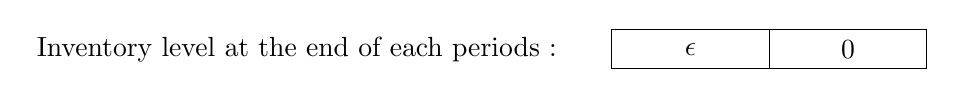
\begin{tikzpicture}
        \draw (-4, .25) node {Inventory level at the end of each periods : };
        \draw (0, 0) rectangle (2, .5) ++(-1, -.25) node {$\epsilon$};
        \draw (2, 0) rectangle (4, .5) ++(-1, -.25) node {$0$};
    \end{tikzpicture}
\end{center}

This allows to compute the total cost like so :
\[
    J = K + h\epsilon +
    \begin{cases}
        K &\textrm{if }\epsilon = 0\\
        0 &\textrm{if }\epsilon = d_2\\
        K &\textrm{if }\epsilon < d_2
    \end{cases}
    = \begin{cases}
        2K+h\epsilon&\textrm{if }\epsilon<d_2\\
        K+hd_2&\textrm{if }\epsilon = d_2
    \end{cases}
\]
Indeed, we always pay at least one order (which corresponds to the first order in period one) and the inventory cost for the remaining items after the first periods (which is $\epsilon$). In the case where $\epsilon = d_2$, we already have ordered enought products to fulfill both the demand of the first period and the demand of the second period, so we don't have to make another order and we don't pay for ordering nothing. Otherwise, we have to order again, so a new $K$ cost has to be paid. We then have two cases :
\begin{itemize}
    \item if $\epsilon < d_2$, then clearly, the minimum is reached by choosing $\epsilon = 0$
    \item if $\epsilon = d_2$, then minimum is $K+hd_2$
\end{itemize}

What this discussion means, is that, in order to choose a value for $\epsilon$ in order to minimize our cost, the only "good" decisions we can make are those of buying once for two periods or buying once at each period but in no case should we buy more in period one and buy again a smaller amount of goods in period two. That's the meaning of the Wagner-Within theorem.

\section{The Silver \& Mill Heuristic}

The Silver-Meal heuristic is a very simple algorithm which relies on the Wagner-Within theorem. It often drives the solution near the real solution which in most cases is acceptable. In fact, the algorithm finds a local minimum of the cost function (instead of a global minimum). Simply sumed up, this heuristic considers incrementing periods of time and looks at whether or not it would be a good idea to buy more than what is needed for that specific period of time. We know from the Wagner-Within theorem that if we buy more than needed, then whe should buy exactely the amount of good sufficient to satisfy the demand of the next period (otherwise it's not worth it). The algorithm computes a series of costs making this kind of assumptions until a local minimum is reached. Here is how it works : let $c(i)$ be the cost we would pay if, starting from the first period, we were to buy as many products as needed to statisfy up to the $i$-th period's demand. Clearly, the cost $c(1)$ is simply $K$ since we only make one order and don't pay for inventory since all our order is consumed by the demand in the first period ($a_1=d_1$). For the second period, the cost $c(2)$ is now the fixed price $K$, since we order once for two periods, to which we have to add the inventory cost we pay for the remaining inventory level after period one which corresponds exactely to $hd_2$. In order to compare $c(1)$ and $c(2)$, we'll focus on the \emph{average} cost that we pay per period of time instead of the absolute value. It holds then that $c(2) = \frac{K+hd_2}{2}$. Similarly, we can compute $c(3)$ as $c(3) = \frac{K + h(d_2+d_3) + hd_3}{3}=\frac{K+hd_2+2hd_3}{3}$ since we order once for the three subsequent periods of time and that we have to pay for inventory in period one (whose inventory level is then $d_2+d_3$) and in period two (whose inventory level is then $d_3$). Continuing like so, and searching for a local minimum, we get the Silver-Mill heuristic for choosing our actions. 

The general formula (which can be recursively demonstrated) for computing the coefficients $c(i)$s is given by 
\[ c(i) = \frac{K+hd_2+2hd_3+\hdots+(i-1)d_i}{i} \] Indeed, we assume paying once in period one, so we pay the order price $K$ just once, then we have to deal with inventory costs. The quantity $d_k$ will remain in the inventory untill period $k$ is reached. So the associated inventory cost is given by $(k-1)hd_k$ since we pay for having it in store in every preceding periods of time. 

The figure (\ref{periodic:local_minimum}) shows how the heuristic works. The algorithm continues to compute total costs (incrementing the number of periods considered) until a local minimum is found. In this example, our action will be to order in the first period for three periods of time since $c(3)$ is a local minimum of our function $J$. Note that, if we had continued to search for lower values we may have eventually found that (in this case), $c(5)$ was more advantageous from an economical point of view and we would have better done to buy all the products for 5 periods instead of four. But in general, this approach gives a really good approximation of the optimal value for the problem and, with respect to the simplicity of the algorithm, it often doesn't worth it to use more advanced and complex models. 

\begin{figure}
    \centering
    \begin{tikzpicture}[scale=1.4]
        \draw[<->] (0, 5.3) node [above] {$c(i)$} |- (7.3, 0) node [right] {$i$};

        \foreach \y in {1,...,5} { \draw[dotted] (0,\y) -- (7,\y); }
        \foreach \x in {1,...,7} { \draw[dotted] (\x,0) -- (\x,5); }

        \draw (1, 4.5) node [draw, cross out] (1) {} ++(0,.5) node {$c(1)$};
        \draw (2, 3) node [draw, cross out] (2) {} ++(0,.5) node {$c(2)$};
        \draw (3, 2) node [draw, cross out] (3) {} ++(0,.5) node {$c(3)$};
        \draw (4, 3.4) node [draw, cross out] (4) {} ++(0,.5) node {$c(4)$};
        \draw (5, 1.5) node [draw, cross out] (5) {} ++(0,.5) node {$c(5)$};
        \draw[dotted, thick] (1) -- (2) -- (3) -- (4) -- (5);

        \draw[red, ->, thick] (3,0) -- (3);
    \end{tikzpicture}
    \caption{\label{periodic:local_minimum}Silver-Mill heuristic example}
\end{figure}

\section{Analysis of the method}

In this last section of this chapter, we would like to discuss on the accuracy, or rather plausibility, of this method. In particular, we will have a look at what happens the demand for each period of time is homogeneous. Let $d$ be that demand. Using the previously established formula, it holds that :
\[
    \begin{split}
        c(n) &= \frac{K+hd+2hd+\hdots+(n-1)hd}{n}\\
            &= \frac{K+\sum_{i=1}^{n-1}ihd}{n}\\
            &= \frac{K+\frac{n(n-1)}{2}}{n}\\
            &= \frac{K}{n} + \frac{nhd}{2} - \frac{hd}{2}
    \end{split}
\]
and let us relax our problem considering the function $c(x)$ where $x$ is no longer discrete but continuous. Derivating this function, we get 
\[
    \begin{cases}
        \frac{dc}{dx} &= -\frac{K}{n^2} + \frac{hd}{2}\\
        \frac{d^2c}{dx^2} &= \frac{K}{n^3} > 0, \forall x\in\mathbb R
    \end{cases}
\]
The second derivative being greater than zero for any $x$ means that the function $c$ is convex. Knowing that, it is legit to compute the minimum of this function by truncating the solution of $\nabla c = 0$ to find the actual minimum of the non-relaxed problem (where $x\in\mathbb N$). Solving this equation we get : \[ \frac{dc}{dx} = 0 \Leftrightarrow x^* = \sqrt\frac{2K}{hd} \]
And since $Q = dn^*$, it holds that \[ Q = dx^* = \sqrt\frac{2kd}h  \] which is the exact same formula which we found in the first part of this course in the deterministic model. 

    \part{Bill of materials}
    \chapter{Model without set-up times}
    Looking back at figure (\ref{intro:production-system}), we realise that we have only been focusing on one part of the global schema. Indeed, we have only dealt with inventory management so far. This part of the course will now focus on what is called "Bill of materials" in which we look at how we can manage the relations between raw materials and final product production.

\section{Model representation and explosion of bill of materials}

The Bill of materials uses a standard representation in terms of graph. The nodes are a set of products : raw materials, final products or temporary products. Temporary products are products which are used to make either other temporary products or final products from either other temporary products or raw materials. The arcs of the graph represents transformations. In figure (\ref{without_st:representation}), the first case where a node $i$ is linked to a node $j$ represents the fact that, somehow, product $i$ is transformed into product $j$, for instance, if we paint a piece of wood (product $i$) it becomes a painted piece of wood (product $j$), or again, if we cut a large piece of iron (product $i$) we transforme it into \emph{several} smaller pieces of iron. The number $n_{ij}$ valuating the arc tells us how many product $i$ we need to produce a single product $j$. If we consider the painting operation, then $n_{ij}=1$, whereas if we consider cutting an iron piece, $n_{ij}\ge 2$ (depending on the situations). The second case represents the fact of assembling products $i$ and $j$ in order to make product $k$. Again, $n_{ik}$ represents the number of product $i$ needed to make one product $k$.

\begin{figure}[h!]
    \centering
    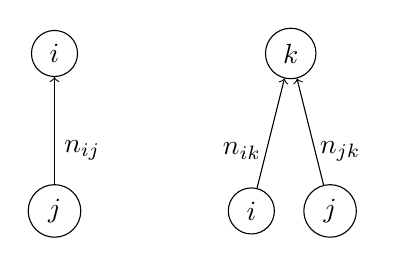
\begin{tikzpicture}
        % first case
        \node[draw, circle] at (0,0) (i) {$i$};
        \node[draw, circle] at (0,-2) (j) {$j$};
        \draw[<-] (i) -- node [below right] {$n_{ij}$} (j);

        % second case
        \node[draw, circle] at (3, 0) (k) {$k$};
        \node[draw, circle] at (2.5, -2) (i2) {$i$};
        \node[draw, circle] at (3.5, -2) (j2) {$j$};
        \draw[->] (i2) -- node[below left] {$n_{ik}$} (k);
        \draw[->] (j2) -- node[below right] {$n_{jk}$} (k);
    \end{tikzpicture}
    \caption{\label{without_st:representation}Bill of materials representation in terms of graph}
\end{figure}

Let's now consider figure (\ref{without_st:first_example}) which shows you a first example of bill of materials and let's extend the notation $n_{ij}$ to any nodes $i$ and $j$ as long as there exists a path from $i$ to $j$ in the graph. Then, $n_{2f}$ represents the number product $2$ needed to produce $1$ final product $f$. How can we compute that value ? It is rather simple : we need $3$ units of product $1$ to produce $1$ unit of product $f$, but we need $2$ unit of product $2$ to produce $1$ unit of product $1$ ; the quantity $n_{2f}$ is then given by $n_{21}\times n_{1f} = 2 \times 3 = 6$, we need $6$ units of procut $2$ to produce $1$ unit of product $f$. In general, the following formula holds : \[ n_{kf} = \prod_{ (i,j)\in Path(k\rightarrow f) } n_{ij} \]

\begin{figure}[h!]
    \centering
    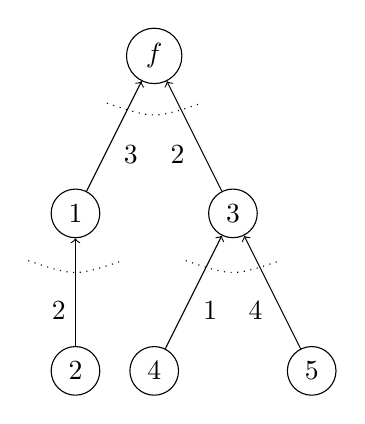
\begin{tikzpicture}
        \draw (0,0) node [draw, circle] (f) {$f$};
        \draw (-1,-2) node [draw, circle] (1) {$1$};
        \draw (-1,-4) node [draw, circle] (2) {$2$};
        \draw (1,-2) node [draw, circle] (3) {$3$};
        \draw (0,-4) node [draw, circle] (4) {$4$};
        \draw (2,-4) node [draw, circle] (5) {$5$};

        \draw[->] (1) -- node (1f) [below right] {3} (f);
        \draw[->] (2) -- node [below left] {2} (1);
        \draw[->] (3) -- node (2f) [below left] {2} (f);
        \draw[->] (4) -- node [below right] {1} (3);
        \draw[->] (5) -- node [below left] {4} (3);

        \draw[dotted] (-.6, -.6) .. controls (0, -.8) .. (.6, -.6);
        \draw[dotted] (-1.6, -2.6) .. controls (-1, -2.8) .. (-.4, -2.6);
        \draw[dotted] (.4, -2.6) .. controls (1, -2.8) .. (1.6, -2.6);
    \end{tikzpicture}
    \caption{\label{without_st:first_example}First example of Bill of Materials}
\end{figure}

It is clear now that if we want to produce a certain number of product $f$ denoted $X_f$, we need to produce at least $X_fn_{if}$ product $i$ so that $X_i\ge X_fn_{if}$. In the following discussion, we will always choose $X_i = X_fn_{if}$ which corresponds to the "conservation of flow" in our system (even though it is not a necessary condition). An other assumption we will make in this chapter, as well as in chapter 2, is that every machine can produce only one kind of product. We will then denote by $i$ both the product and the machine producing it. 

Considering machine $i$, let $\mu_i$ be the maximum speed for producing one product, expressed as items/unit of time, and we define $u_i$ as the "utilization of the resource $i$" which equals : \[ u_i = \frac{X_fn_{if}}{\mu_i}\le 1, \forall i \] Using that definition, it holds that \[ X_f\le\frac{\mu_i}{n_{if}}, \forall i\Leftrightarrow X_f\le\min_i\left( \frac{\mu_i}{n_{if}} \right) \overset{\Delta}{=} X_f^{max} \] where $X_f^{max}$ is the maximum rate at which we can produce product $f$ with respect to the machines we use to produce it. The bottleneck machine(s) can be computed as $\textrm{argmin}_i\left( \frac{\mu_i}{n_{if}} \right)$. This (or these) machine(s) is (are) the one(s) which prevents us from producing more, at a higher rate. 

\section{Production time}

Given a machine $i$, we can compute the operation time needed to produce one item of product $i$ which is simple \[ T_{oi} = \frac{1}{\mu_i} \] We then enhance figure (\ref{without_st:first_example}) with those operation times as a valuation of the arcs. Figure (\ref{without_st:with_toi}) shows such a representation. The operation time has been added as the second element of a couple. The first element will be dealt with in chapter two of this section. The maximum rate $X_f^{max}$ at which we can produce our final product is then given by \[ X_f^{max} = \min_i\left( \frac{1}{T_{oi}n_{if}} \right) \]

\begin{figure}[h!]
    \centering
    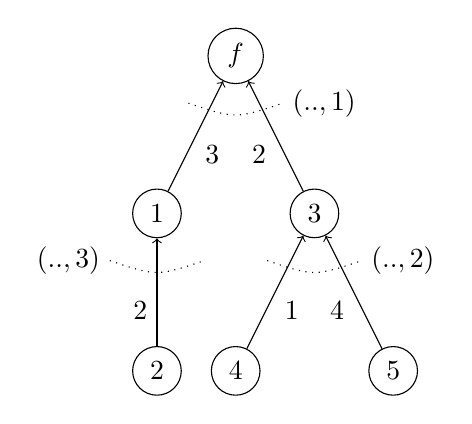
\begin{tikzpicture}
        \draw (0,0) node [draw, circle] (f) {$f$};
        \draw (-1,-2) node [draw, circle] (1) {$1$};
        \draw (-1,-4) node [draw, circle] (2) {$2$};
        \draw (1,-2) node [draw, circle] (3) {$3$};
        \draw (0,-4) node [draw, circle] (4) {$4$};
        \draw (2,-4) node [draw, circle] (5) {$5$};

        \draw[->] (1) -- node (1f) [below right] {3} (f);
        \draw[->] (2) -- node [below left] {2} (1);
        \draw[->] (3) -- node (2f) [below left] {2} (f);
        \draw[->] (4) -- node [below right] {1} (3);
        \draw[->] (5) -- node [below left] {4} (3);

        \draw[dotted] (-.6, -.6) .. controls (0, -.8) .. (.6, -.6) node[right] {$(.., 1)$};
        \draw[dotted] (-1.6, -2.6) node[left] {$(.., 3)$} .. controls (-1, -2.8) .. (-.4, -2.6);
        \draw[dotted] (.4, -2.6) .. controls (1, -2.8) .. (1.6, -2.6) node[right] {$(.., 2)$};
    \end{tikzpicture}
    \caption{\label{without_st:with_toi}First example of Bill of Materials}
\end{figure}

Let's start by computing the $n_{if}$ quantities for all $i$, we get :
\[
    \begin{aligned}[l]
        n_{1f} &= 3 & n_{3f} &= 2 & n_{5f} &= 4\times 2 = 8\\
        n_{2f} &= 2\times 3 = 6 & n_{4f} &= 1\times 2 = 2\\
    \end{aligned}
\]
then we can find $X_f^{max}$ as well as the bottleneck machine by doing the following
\[
    \begin{split}
        X_f^{max} &= \min_i\left( \frac{1}{T_{oi}n_{if}} \right)\\
                  &= \min\left( \frac{1}{1\times 3} , \frac{1}{3\times 6} , \frac{1}{1\times 2} , \frac{1}{2\times 2} , \frac{1}{2\times 4} \right)\\
                  &= \min\left( \frac{1}{3} , \frac{1}{18} , \frac{1}{2} , \frac{1}{4} , \frac{1}{8} \right)\\
                  &= \frac{1}{18}\\
                  \\
        bottleneck &= \textrm{arg}\min_i\left( \frac{1}{T_{oi}n_{if}} \right) = 2\\
    \end{split}
\]
Note that, in this case, the bottleneck machine is the one with the highest operation time. This is NOT a general rule, and it's easy to find a counter example : consider a final product $f$ which is made by assembling a hundred small pieces with one big one. Clearly, even if the machine which produces the small pieces is efficient, it is \emph{possible} that making a hundred of these pieces may be longer than producing one other piece, even bigger. But again, this isn't always the case. The only way to solve for the bottleneck machine problem is to look at both the operation time and the number of products required to produce the final product. 

\section{Batch production}

A batch $b_i$ can be defined as the number of items $i$ the machine produces without interuption before releasing it to other machines. Let's suppose that we want to produce a batch of final product $b_f$, how much time do we need to do it ? In this section, we will try to answer that question considering that our batch sizes are $b_i = b_fn_{if}$, which is not necessary, but simpler. In general however, you often have external constraints (linked to the technology you use for example) which imposes a minimum batch size or a maximum batch size, so that : 
\[ b_i^{min} \le b_i \le b_i^{max}, \forall i \]
From that constraint, we can deduce the following
\[
    \begin{split}
        \Rightarrow & b_i^{min} \le b_fn_{if} \le b_i^{max}, \forall i \\
        \Rightarrow & \frac{b_i^{min}}{n_{if}} \le b_i \le \frac{b_i^{max}}{n_{if}}, \forall i\\
        \Rightarrow & \max_i\left( \frac{b_i^{min}}{n_{if}} \right) \le b_f \le \min_i\left( \frac{b_i^{max}}{n_{if}} \right)
    \end{split}
\]
Since the batch size $b_f$ has to be an integer, we have to make sure that this interval contains at least on integer value, otherwise, we cannot use $b_i = b_fn_{if}$ as a batch size. 

Considering that relation to hold however, we can compute the production time for a given batch as \[ T_{i,prod}(b_i) = T_{oi}b_i = T_{oi}b_fn_{if} \] which now allows us to compute the time it takes to go from one raw material (a leaf of the tree in our graph representation) to the final product (root of tree). Considering $\mathcal P_k$ as the path going from the raw material $k$ to the final product in our graph, it holds that \[ T_{\mathcal P_k} = \sum_{j\in\mathcal P_k}T_{j,prod}(b_j) = b_f\sum_{j\in\mathcal P_k} T_{oj}n_{jf} \] This relation tells us about how much time we would need to produce a batch of final product $b_f$ since \[ T_{prod}(b_f) = \max_{\mathcal P_k}\left( T_{\mathcal P_k}(b_f) \right) \]

Up to now, we have considered choosing a batch size $b_f$ and compute the time needed to produce it. But we can as well use the established formulas in the other way to compute the maximum batch size allowed in order respect a certain constraint on production time. For instance, let's say we want to respect the condition $T_{prod}(b_f) \le T^{max}$ meaning that we do not want to produce more than $T^{max}$ units of time. Then it still holds that 
\[
    \begin{split}
        T_{prod}(b_f) \le T^{max}
            &\Leftrightarrow b_f\max_{\mathcal P_k}\left( b_f\sum_{j\in\mathcal P_k} T_{oj}n_{jk} \right) \le T^{max}\\
            &\Leftrightarrow b_f \le \frac{T^{max}}{ \max_{\mathcal P_k}\left( \sum_{j\in\mathcal P_k} T_{oj}n_{jk} \right) }
    \end{split}
\] which tells us about the maxumum size we can use for a batch in order to fullfill that constraint. 

One final consideration is to be taken regarding the rotation of batches. Let's say we want to produce $X_f^* \le X_f^{max}$ final products. We introduce the variable $D$ as the difference in time between the moment a batch is produced and the moment a subsequent batch is produced so that \[ X_f^* = \frac{b_f}{D} \] (number of items of the final product over the time of a "period" of production) The figure (\ref{without_st:cycle}) illustrates this notion.

\begin{figure}[h!]
    \centering
    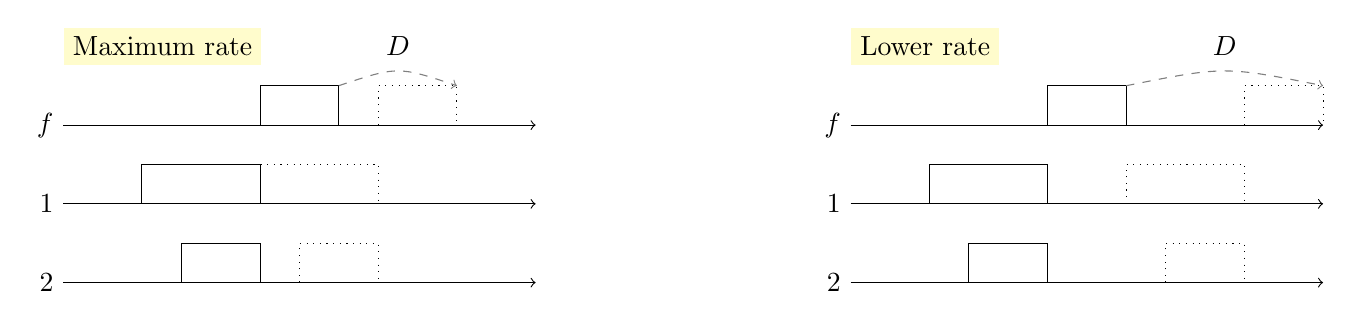
\begin{tikzpicture}

    % maximum rate
    \draw (0, 1) node [right, fill=yellow!20] {Maximum rate};

    \draw[->] (0,0) node[left] {$f$} -- (6,0);
    \draw (2.5, 0) rectangle (3.5, .5);
    \draw[dotted] (4, 0) rectangle (5, .5);

    \draw[->] (0,-1) node[left] {$1$} -- (6,-1);
    \draw (1, -1) rectangle (2.5, -.5);
    \draw[dotted] (2.5, -1) rectangle (4, -.5);

    \draw[->] (0,-2) node[left] {$2$} -- (6,-2);
    \draw (1.5, -2) rectangle (2.5, -1.5);
    \draw[dotted] (3, -2) rectangle (4, -1.5);

    \draw[->, dashed, gray] (3.5, .5) .. controls (4.25, .75) .. (5, .5);
    \draw (4.25, 1) node {$D$};
    
    % lower rate
    \draw (10, 1) node [right, fill=yellow!20] {Lower rate};
    \draw[->] (10,0) node[left] {$f$} -- (16,0);
    \draw (12.5, 0) rectangle (13.5, .5);
    \draw[dotted] (15, 0) rectangle (16, .5);

    \draw[->] (10,-1) node[left] {$1$} -- (16,-1);
    \draw (11, -1) rectangle (12.5, -.5);
    \draw[dotted] (13.5, -1) rectangle (15, -.5);

    \draw[->] (10,-2) node[left] {$2$} -- (16,-2);
    \draw (11.5, -2) rectangle (12.5, -1.5);
    \draw[dotted] (14, -2) rectangle (15, -1.5);

    \draw[->, dashed, gray] (13.5, .5) .. controls (14.75, .75) .. (16, .5);
    \draw (14.75, 1) node {$D$};

    \end{tikzpicture}
    \caption{\label{without_st:cycle}GANTT diagram with production cycle}
\end{figure}

    \chapter{Model with set-up time considerations}
    \section{Taking setup time into account}

\section{Finding the bottleneck machine(s)}

    \chapter{Arbitrary batch sizing ($b_i \ne b_fn_{if}$)}
    So far, we have built a model considering operation time and setup times to for each machine. Doing that, we made an assumption that for any $i$ we would choose the batch production size of product $i$ following the rule $b_i = b_fn_{if}$. We saw that (1) this is not mandatory (but simpler from the point of view of calculations) and that (2) it is not always feasible. In this chapter, we will discuss the case when $b_i \ne b_fn_{if}$. In the first chapter of this part, we established the following formula : 
\[ X_f^{max}(\underline b) = \min_i\left( \frac{\mu_i}{n_{n_{if}}}\right) = \min_i\left( \frac{b_i}{T_{si} + T_{oi}b_i} \middle/ n_{if} \right) \] If we want to produce at a minimum production rate $X_f^*$ we can now compute the minimum batch size on machine $i$ like so \[
    \begin{split}
        X_f^{max}(\underline b) \ge X_f^*
            &\Leftrightarrow \frac{b_i}{T_{si}+T_{oi}b_i}\ge X_f^*n_{if},\forall i\\
            &\Leftrightarrow b_i\ge X_f^*n_{if}T_{si} + X_f^*n_{if}T_{oi}b_i,\forall i\\
            &\Leftrightarrow b_i\ge \frac{X_f^*n_{if}T_{si}}{1 - X_f^*n_{if}T_{oi}}, \forall i
    \end{split}
\]
Futhermore, we know that the production rate for machine $i$ can be computed as $X_i^*=X_f^*n_{if}$ and that the "production" cycle is given by $D_i^*=\frac{b_i}{X_i^*}$. However, how can we draw a GANTT diagram of such a production plan ?

\section{The Kanban organisation}

In this section, we will try to compute the overall "production cycle". That is, from which point in time can we repeat the production of a batch of size $b_i$ for machine $i$. Since every machine can now choose an arbitrary batch size, how can we plan our production ? Well, for it to be repeatable, the overall production cycle $D$ has to be a multiple of each particular machine production cycle $D_i^*$. The minimum one being the \emph{minimum common multiple} of each $D_i$ of the machines. Thus, we have a lower bound for the production cycle which is \[ D^* = \underset{i}{\textrm{mcm}}(D_i^*) \]Note that the \emph{minimum common multiple} doesn't have to be an integer, for example : $\textrm{mcm}\left( \frac{1}{2} ; \frac{1}{4} \right) = \frac{1}{2}$. 

Given these numbers, we can easily input how many items of product $i$ are produced during a whole period $D^*$ since $D^*/D_i^*$ (which is integer) equals the number of batches produced in the time period $D^*$, we get that \[ \#items(i) = \left( \frac{D^*}{D_i^*} \right)b_i \] which can be written in a similar way by substituting $D_i^*$ by its expresion in terms of $b_i$, $n_{if}$ and $X_f^*$ as previously introduced : \begin{equation} \#items(i) = \dfrac{D^*}{ \frac{\cancel{b_i}}{X_f^*n_{if}} }\cancel{b_i} = (D^*X_f^*)n_{if} \label{giving_up:eq1} \end{equation} Finally, since $n_{ff} = 1$, it holds that $\#items(f) = D^*X_f^*$, which makes relation (\ref{giving_up:eq1}) somehow analogous to our initial relation $b_i = b_fn_{if}$.

\begin{wrapfigure}[14]{l}{4cm}
    \centering
    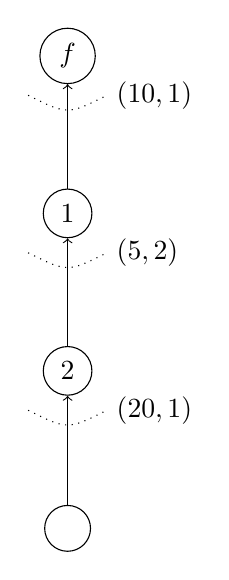
\begin{tikzpicture}
        \draw (0, 0) node[draw, circle] (f) {$f$};
        \draw (0, -2) node[draw, circle] (1) {$1$};
        \draw (0, -4) node[draw, circle] (2) {$2$};
        \draw (0, -6) node[draw, circle] (RM) {$\vphantom{j}$};

        \draw[dotted] (-.5, -.5) .. controls (0, -.75) .. (.5, -.5) node[right] {$(10, 1)$};
        \draw[dotted] (-.5, -2.5) .. controls (0, -2.75) .. (.5, -2.5) node[right] {$(5, 2)$};
        \draw[dotted] (-.5, -4.5) .. controls (0, -4.75) .. (.5, -4.5) node[right] {$(20, 1)$};

        \draw[<-] (f) -- (1);
        \draw[->] (2) -- (1);
        \draw[<-] (2) -- (RM);
    \end{tikzpicture}
    \caption{\label{giving_up:bom1}Example}
\end{wrapfigure}

But let's have an example in order to understand better how we can draw our gantt. Consider figure (\ref{giving_up:bom1}) and a minimum production rate $X_f^* = \frac{1}{3}$. We can easily compute the minimum batch size resulting of that constraint using the previously cited formula like so :
\[
    \begin{split}
        b_f &\ge \frac{\frac{1}{3}.1.10}{1-\frac{1}{3}.1.1} = 5\\
        b_1 &\ge \frac{\frac{1}{3}.1.5}{1 -\frac{1}{3.1.2}} = 5\\
        b_2 &\ge \frac{\frac{1}{3}.1.20}{1-\frac{1}{3}.1.1} = 10
    \end{split}
\]
These lower bounds tell us about the minimum batch size we have to use in order to produce at the minimum rate $X_f^*=\frac{1}{3}$. Thus, we can use greater batch sizes like the following : $b_f = 6$, $b_1 = 5$ and $b_2 = 10$. Using this choice, we can compute each machine's production cycle like so 
\[
    D_f^* = \frac{6}{\frac{1}{3}.1} = 18 = 2.3^2 \textrm{ ; }
    D_1^* = \frac{5}{\frac{1}{3}.1} = 15 = 3.5 \textrm{ ; }
    D_2^* = \frac{10}{\frac{1}{3}} = 30 = 2.3.5
\]
From which we can now deduce the minimum common multiple which is the minimum production cycle for the overall plan : $D^* = 2.3^2.5 = 90$. Assuming these results, you will find in figure (\ref{giving_up:gant1}) the GANTT representation of two production cycles.

\begin{figure}[h!]
    \centering
    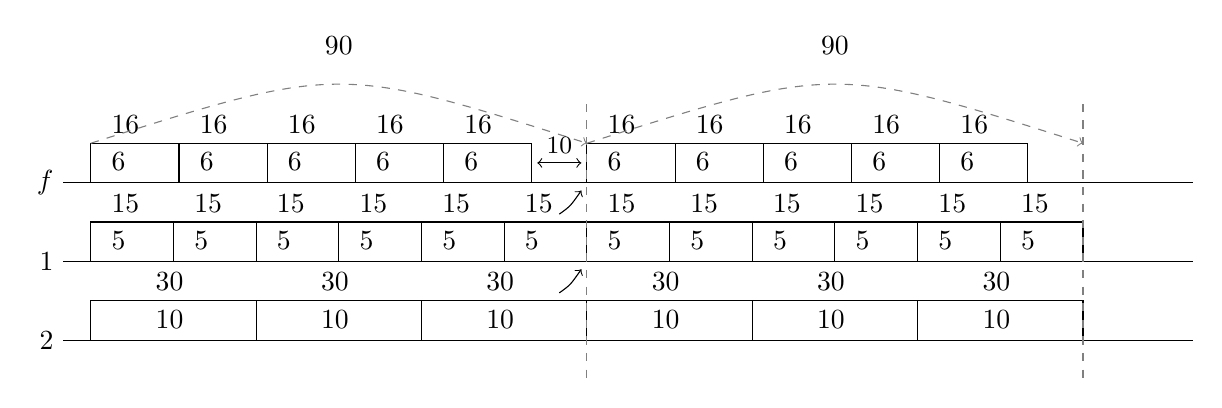
\begin{tikzpicture}[xscale=.07, yscale=.5]
        \draw (-5,0) node[left] {$f$} -- (200, 0);
        \foreach\cycle in {0, 1}
            \foreach \x in {0,...,4} {
                \draw (\cycle * 90 + \x*16, 0) rectangle (\cycle * 90 + \x*16 + 16, 1);
                \draw (\cycle * 90 + \x*16 + 2, 1) node[above right] {$16$};
                \draw (\cycle * 90 + \x*16 + 2, 1) node[below right] {$6$};
            }

        \draw (-5,-2) node[left] {$1$} -- (200, -2);
        \foreach\cycle in {0, 1}
            \foreach \x in {0,...,5} {
                \draw (\cycle * 90 + \x*15, -2) rectangle (\cycle * 90 + \x*15 + 15, -1);
                \draw (\cycle * 90 + \x*15 + 2, -1) node[above right] {$15$};
                \draw (\cycle * 90 + \x*15 + 2, -1) node[below right] {$5$};
            }
        
        \draw (-5,-4) node[left] {$2$} -- (200, -4);
        \foreach\cycle in {0, 1}
            \foreach \x in {0,...,2} {
                \draw (\cycle * 90 + \x*30, -4) rectangle (\cycle * 90 + \x*30 + 30, -3);
                \draw (\cycle * 90 + \x*30 + 10, -3) node[above right] {$30$};
                \draw (\cycle * 90 + \x*30 + 10, -3) node[below right] {$10$};
            }

        \draw[dashed, gray] (90, 2) -- (90, -5);
        \draw[dashed, gray] (180, 2) -- (180, -5);

        \draw[dashed, gray, ->] (0, 1) .. controls (45, 3) .. (90, 1);
        \draw[dashed, gray, ->] (90, 1) .. controls (135, 3) .. (180, 1);
        \draw (45, 3) node[above] {$90$};
        \draw (135, 3) node[above] {$90$};

        \draw[->] (85, -.8) .. controls (87, -.6) .. (89, -.2);
        \draw[->] (85, -2.8) .. controls (87, -2.6) .. (89, -2.2);
        \draw[<->] (81, .5) -- node[above] {\small $10$} (89, .5);
    \end{tikzpicture}
    \caption{\label{giving_up:gant1}Resulting GANTT diagram}
\end{figure}

However, as depicted in figure (\ref{giving_up:gant1}), one may have noticed that we did not fully respect the dependency of product $1$ over product $2$, nor of $f$ over $1$. In fact, it is not possible to draw such a GANTT. To avoid this, we assume the existence of queues in front of each machine and that from now on, the objective for every machine is to fill the queue in front of it when it is emptied. This way of reasonning is called "pull production" since the information flow goes from right to left, whereas in the previous chapters we were referencing to "push production" since it was the raw material which determined when the following tasks could begin. In this view of the production line, every machine starts producing a batch as soon as the queue in front of him is empty. It is called as well KANBAN organisation. 

\section{Using Kanban with $b_i = b_fn_{if}$}

Studying this new kind of systems, we have discovered a new pattern for production scheduling. In this section, we will have a look at what happens if we apply the KANBAN organisation to the situations in which $b_i = b_fn_{if}$. Of course, we have $X_f^* = b_f^*$ which gives us, for machine $i$, a production cycle of \[ D_i^* = \frac{b_fn_{if}}{X_f^*n_{if}} = \frac{b_f}{X_f^*} \] which does not depend on $i$. Computing the overall production rate is trivial since the \emph{minimum common multiple} of a set of identical numbers $D_i^*$ is simply given by $D_i^*$. So that $D^* = D_i^*, \forall i$ since they are the same. 

Using figure (\ref{giving_up:bom1}) again with the same production rate ($\frac{1}{3}$), we can compute $b_f^*$ easily like before. This yields $b_f^* = 10$. Let's say we decide to use $b_f = 12$. Then we can compute the production cycle as $D^* = \frac{12}{\frac{1}{3}} = 36$ (and of course $D^* = D_i^*$) and we can draw, as in figure (\ref{giving_up:gant2}), the GANTT diagram of such a plan. 

\begin{figure}[h!]
    \centering
    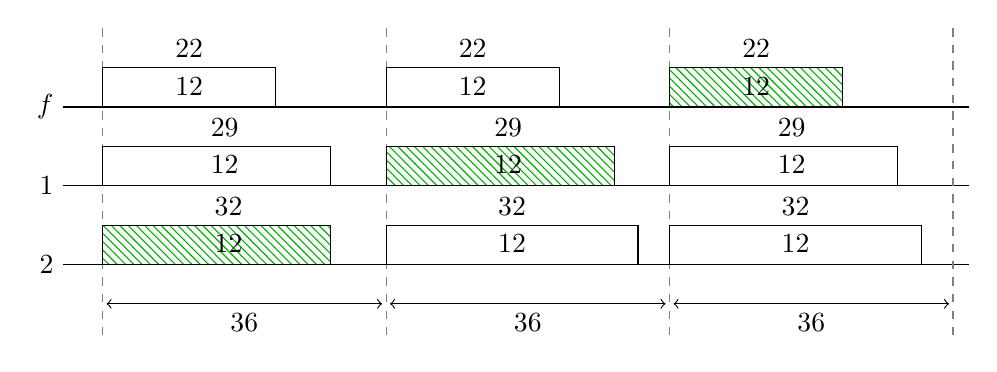
\begin{tikzpicture}[xscale=.1, yscale=.5]
        \draw (-5,0) node[left] {$f$} -- (110, 0);
        \draw (-5,-2) node[left] {$1$} -- (110, -2);
        \draw (-5,-4) node[left] {$2$} -- (110, -4);

        \foreach \cycle in {0,...,3} \draw[dashed, gray] (\cycle * 36, 2) -- (\cycle * 36, -6);

        \draw (0,0) rectangle (22, 1);
        \draw (36,0) rectangle (58, 1);
        \draw[pattern=north west lines, pattern color=black!30!green] (72,0) rectangle (94, 1);

        \draw (0,-2) rectangle (29, -1);
        \draw[pattern=north west lines, pattern color=black!30!green] (36,-2) rectangle (65, -1);
        \draw (72,-2) rectangle (72 + 29, -1);

        \draw[pattern=north west lines, pattern color=black!30!green] (0,-4) rectangle (29, -3);
        \draw (36,-4) rectangle (36 + 32, -3);
        \draw (72,-4) rectangle (72 + 32, -3);

        \foreach \cycle in {0,...,2} {
            \draw[<->] (\cycle * 36 + .5, -5) -- (\cycle * 36 + 36 - .5, -5);
            \draw (\cycle * 36 + 18, -5) node[below] {$36$};
            
            \draw (\cycle * 36 + 11, 1) node[below] {$12$};
            \draw (\cycle * 36 + 15.5, -1) node[below] {$12$};
            \draw (\cycle * 36 + 16, -3) node[below] {$12$};

            \draw (\cycle * 36 + 11, 1) node[above] {$22$};
            \draw (\cycle * 36 + 15.5, -1) node[above] {$29$};
            \draw (\cycle * 36 + 16, -3) node[above] {$32$};
        }

    \end{tikzpicture}
    \caption{\label{giving_up:gant2}GANTT diagram using batch size $b_f = 12$}
\end{figure}

If we assume to start the production with empty queues in front of each machine, what would be the time needed to produce the first batch ? Well, as represented by the green rectangles in figure (\ref{giving_up:gant2}), we would roughly need to wait as many production cycles as there are levels in the bill of materials (which means, product dependencies). Thus, the following formula 
\[
    \textrm{Production time of the first batch} \approx \textrm{production cycle}\times\textrm{number of levels of BoM}
\]
In our example, this formula gives us $3\times 36 = 108$, when the real result is $94$.

    \chapter{Fullfillement of an order}
    Up to this chapter, our focus has been on the fullfillment of a constraint given in terms of production rate and production time. In this part of the course, we will change our main objective by adding a constraint on the number of items to be produced. Still we will have a minimum rate to be performed, stil we will have a production time limit not to be crossed, but the objective now becomes to produce exactely $N$ final products and to plan the production accordingly. 

\section{Given that $b_i = b_fn_{if}$}

\subsection{Push systems}

We know, from the previous chapters, that the production time can be computed as \[ T_{prod}(b_f) = \max_{\mathcal P_k}\left( \sum_{i\in\mathcal P_k}(T_{si} + b_fT_{oi}n_{if}) \right) \] but it is worthy to notice that the time to seperately produce two batches of size $b_f$ does not equal the double time we would need to produce one batch of size $b_f$. More formally, we are saying that $T_{prod}(2.b_f)|_{b_f}\ne 2T_{prod}(b_f)$ in the sense that figure (\ref{produced_i:2bf}) represents. In fact, we do not need for a whole "production cycle" to be finished to begin with another one. Indeed, we can begin a new cycle as soon as the "longest" machine has done its work (i.e. the bottleneck machine). The following formula holds instead : \[ \left. T_{prod}(2.b_f) \right|_{b_f} = T_{prod}(b_f) + T_b(b_f) \] where $\left. T_{prod}(2.b_f) \right|_{b_f}$ represents the time needed to produce $2.b_f$ items knowing that the batch size is $b_f$ and where $T_b(b_f)$ is the time which is needed, by the bottleneck machine (hence $T_b$ for bottleneck) to produce a bacth of size $b_f$. This formula can, for sure, be generalized as \begin{equation} \left. T_{prod}(K.b_f) \right|_{b_f} = T_{prod}(b_f) + (K-1)T_b(b_f) \label{produced_i:tprod} \end{equation}

\begin{figure}[h!]
    \centering
    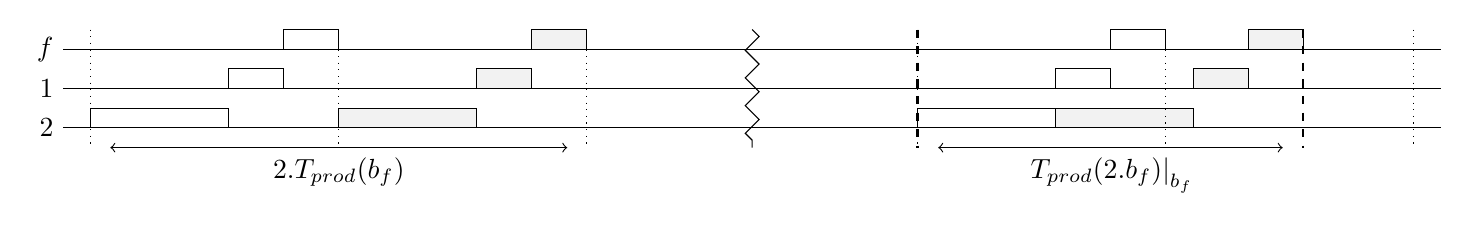
\begin{tikzpicture}[xscale=.7, yscale=.5]
        \draw (0,0) node[left] {$f$} -- (25, 0);
        \draw (0,-1) node[left] {$1$} -- (25, -1);
        \draw (0,-2) node[left] {$2$} -- (25, -2);
        \draw[decorate, decoration=zigzag] (12.5, .5) -- (12.5, -2.5);

        % left
        \draw (.5, -2) rectangle (3, -1.5);
        \draw (3, -1) rectangle (4, -.5);
        \draw (4, 0) rectangle (5, .5);

        \draw[fill=gray!10] (5, -2) rectangle (7.5, -1.5);
        \draw[fill=gray!10] (7.5, -1) rectangle (8.5, -.5);
        \draw[fill=gray!10] (8.5, 0) rectangle (9.5, .5);

        \draw[dotted] (.5, .5) -- (.5, -2.5) node[right] (l1) {};
        \draw[dotted] (5, .5) -- (5, -2.5);
        \draw[dotted] (9.5, .5) -- (9.5, -2.5) node[left] (l2) {};

        \draw[<->] (l1) -- node[below] {$2.T_{prod}(b_f)$} (l2);

        % right
        \draw (15.5, -2) rectangle (18, -1.5);
        \draw (18, -1) rectangle (19, -.5);
        \draw (19, 0) rectangle (20, .5);

        \draw[fill=gray!10] (18, -2) rectangle (20.5, -1.5);
        \draw[fill=gray!10] (20.5, -1) rectangle (21.5, -.5);
        \draw[fill=gray!10] (21.5, 0) rectangle (22.5, .5);

        \draw[dotted] (15.5, .5) -- (15.5, -2.5);
        \draw[dashed, thick] (15.5, .5) -- (15.5, -2.5) node[right] (r1) {};
        \draw[dashed, thick] (22.5, .5) -- (22.5, -2.5) node[left] (r2) {} ;
        \draw[dotted] (20, .5) -- (20, -2.5);
        \draw[dotted] (24.5, .5) -- (24.5, -2.5);

        \draw[<->] (r1) -- node[below] {$\left. T_{prod}(2.b_f)\right|_{b_f}$} (r2);

    \end{tikzpicture}
    \caption{\label{produced_i:2bf}}
\end{figure}

\subsubsection{A first example}

However, the above formula holds for a given bottleneck machine. But we do know that the bottleneck machine depends on the batch size which has been chosen \textit{a priori} : given a batch size $b_f$, we can comptue the production time $T_{prod}(K.b_f)|_{b_f}$. But how can we choose $b_f$ with constraints on the production rate, on the overall production time, and, as well, on the number of items to be produced ? This is not an easy question actually, so let's take an example in order to better understand where the difficulty lies. 

\begin{wrapfigure}[12]{r}{5cm}
    \centering
    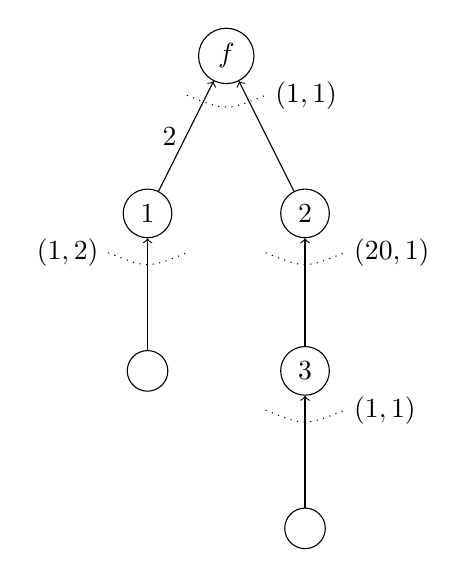
\begin{tikzpicture}
        \draw (0,0) node[draw, circle] (f) {$f$};
        \draw (-1, -2) node[draw, circle] (1) {$1$};
        \draw (-1, -4) node[draw, circle] (RM1) {$\vphantom{1}$};

        \draw (1, -2) node[draw, circle] (2) {$2$};
        \draw (1, -4) node[draw, circle] (3) {$3$};
        \draw (1, -6) node[draw, circle] (RM2) {$\vphantom{1}$};

        \draw[->] (RM1) -- (1);
        \draw[->] (1) -- node[left] {$2$} (f);

        \draw[->] (RM2) -- (3);
        \draw[->] (3) -- (2);
        \draw[->] (2) -- (f);

        \draw[dotted] (-.5, -.5) .. controls (0, -.7) .. (.5, -.5) node[right] {$(1, 1)$};
        \draw[dotted] (-1.5, -2.5) node[left] {$(1, 2)$} .. controls (-1, -2.7) .. (-.5, -2.5);
        
        \draw[dotted] (.5, -2.5) .. controls (1, -2.7) .. (1.5, -2.5) node[right] {$(20, 1)$};
        \draw[dotted] (.5, -4.5) .. controls (1, -4.7) .. (1.5, -4.5) node[right] {$(1, 1)$};
    \end{tikzpicture}
    \caption{\label{produced_i:example1}Example BoM}
\end{wrapfigure}

Let's consider the Bill of Material depicted in figure (\ref{produced_i:example1}) with the following constraints : \begin{enumerate}
    \item Minimum production rate of $X_f^* = \frac{1}{5}$
    \item Maximum production time for a batch $\bar T = 80$
    \item Number of items to be produced $N = 200$
\end{enumerate} We are very used to the first two constraints. The first one gives us a lower bound for the batch size in order for the production rate to be feasible. The second one gives us an upper bound so that the production time of a batch is not greater than the time limit. Computing these bounds is rather easy and we will not discuss them : 
\[
    \begin{split}
        b_f^* &= \max_i\left( \frac{X_f^*T_{si}}{1-X_f^*T_{oi}n_{if}} \right)\\
              &= \max\left(
                    \frac{ \frac{1}{5} . 1 }{1 - \frac{1}{5} . 1 } ;
                    \frac{ \frac{1}{5} . 1 }{1 - \frac{1}{5} . 2 . 2 } ;
                    \frac{ \frac{1}{5} . 20 }{1 - \frac{1}{5} . 1 . 1 } ;
                    \frac{ \frac{1}{5} . 1 }{1 - \frac{1}{5} . 1 . 1 }
                  \right)\\
              &= 5\\
        \bar b_f &= \min_{\mathcal P_k}\left( \frac{\bar T - \sum_{i\in\mathcal P_k}T_{si}}{\sum_{i\in\mathcal P_k}T_{oi}n_{if}}\right)\\
                 &= \min\left(
                        \frac{80 - ( 1 + 1 )}{ 2.2 + 1.1 } ;
                        \frac{80 - ( 1 + 20 + 1 )}{ 1.1 + 1.1 + 1.1 } ;
                    \right)\\
                 &= 15.6
    \end{split}
\]

Which tells us that we need to choose our batch size so that $b_f\in [ 5, 15 ]$. Since we want to produce $N=200$ items, we should repeat a certain number of times the production of such bacthes untill we reach $200$ items. On possible way would be to produce $40$ times a batch of $5$ items (since $40\times 5 = 200$), or produce $25$ times batches of $8$ (since again $25\times 8=200$). In fact, the only multiples of $200$ witin the interval $[5, 15]$ are $\{ 5, 8, 10 \}$. Let's study each one of these cases !

For each cases, we can write the equation (\ref{produced_i:tprod}) as \[
    \begin{split}
        T_{prod}(200)|_{bf=5} &= T_{prod}(5) + 39.T_b(5)\\
        T_{prod}(200)|_{bf=8} &= T_{prod}(8) + 39.T_b(10)\\
        T_{prod}(200)|_{bf=10} &= T_{prod}(8) + 39.T_b(10)\\
    \end{split}
\] where $T_{prod}(b_f)$ can be computed as \[
    T_{prod}(b_f) = \max_{\mathcal P_k}\left( \sum_{i\in\mathcal P_k} ( T_{si} + T_{oi}n_{if} ) \right) = \max ( 2 + 5.b_f ; 22 + 3.b_f )
\] and \[ T_b(b_f) = \max( 1 + 1.b_f ; 1 + 2.2.b_f ; 20 + 1.b_f ; 1 + 1.b_f ) = \max( 1 + 4b_f ; 20 + b_f ) \]

Using these formulas, we easily get the following results : \begin{center}
    \begin{tabular}{|c|c|c|c|}
        \hline
        $b_f$ & $T_{prod}(b_f)$ & $T_b(b_f)$ & $T_{prod}(200)|_{b_f}$\\\hline
        $5$ & $37$ & $25$ & $1012$ \\\hline
        $8$ & $46$ & $33$ & $838$ \\\hline
        $10$ & $52$ & $41$ & $831$ \\\hline
    \end{tabular}
\end{center} Which means that, for this way of producing $200$ items, using a batch size of $10$ items is the quicker (it turns out to be the biggest batch size but this is just a particular case). However, there are other ways of getting to $200$ ! For example, we may want to produce $13$ batches of $15$ and a batch of $5$, since $200 = 13\times 15 + 5$. Looking at figure (\ref{produced_i:gant}), we realise that we can compute the time needed to produce $200$ items in that way by first computing the time to produce $13$ bacthes of $15$ and then add the difference between the needed time to produce a batch of $5$ and the time at which the bottleneck machine can start.

We get that : \[
    \begin{split}
        T_{prod}(15) &= 77\\
        T_b(15) &= 61\\
        T_{prod}(195)|_{bf=15} &= 77 + 12.61 = 809\\
        T_{prod}(5) &= 37\\
        T_b(5) &= 25
    \end{split}
\] And, it holds that the delay represented by the red arrow in figure (\ref{produced_i:gant}) can be computed as the production time of the bottleneck machine $T_b(5)$ minus the production time of machine $f$, which yields $25 - 16 = 9$. We can now compute the final, overall, production time which is : $809 + 9 + 6 = 824$ ! Which is less than what we had previously found. 

\begin{figure}[h!]
    \centering
    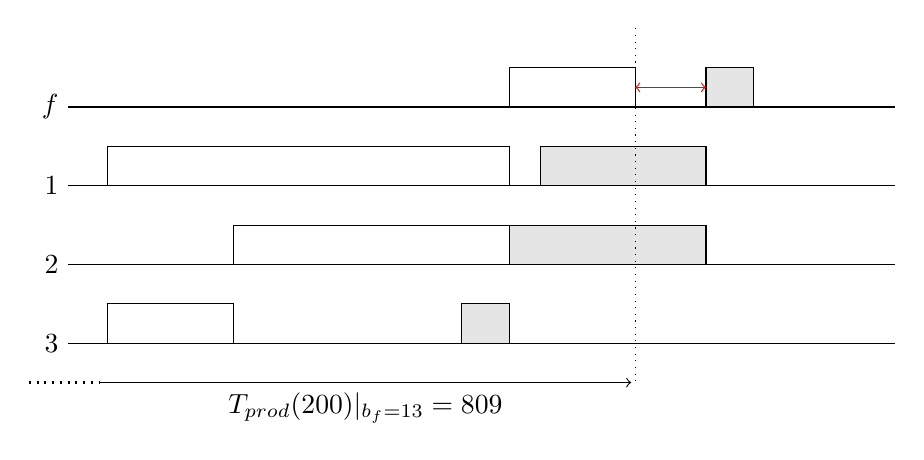
\begin{tikzpicture}[xscale=.1]
        \foreach \y/\m in {0/$f$, -1/$1$, -2/$2$, -3/$3$} \draw (-5,\y) node[left] {\m} -- (100, \y);

        \draw (0,-3) rectangle (16, -2.5);
        \draw (16,-2) rectangle (16 + 35, -1.5);
        \draw (0,-1) rectangle (51, -.5);
        \draw (51, 0) rectangle (51 + 16, .5);

        \draw[fill=gray!20] (51, -2) rectangle (51 + 25, -1.5);
        \draw[fill=gray!20] (51 + 25 - 21, -1) rectangle (51 + 25, -.5);
        \draw[fill=gray!20] (51 - 6, -3) rectangle (51, -2.5);
        \draw[fill=gray!20] (51 + 25, 0) rectangle (51 + 25 + 6, .5);

        \draw[dotted] (67, 1) -- (67, -3.5);

        \draw[->] (-1, -3.5) -- node[below] {$T_{prod}(200)|_{b_f = 13} = 809$} (66.5, -3.5);
        \draw[dotted, thick] (-10, -3.5) -- (-1, -3.5);
        
        \draw[<->, red] (67, .25) -- (67 + 9, .25);
    \end{tikzpicture}
    \caption{\label{produced_i:gant}GANT diagram corresponding to the production of $200 = 13\times 15 + 5$ items}
\end{figure}

Finding the optimal batch size is not easy to be done by hand and we usually use approximation techniques to find a solution. 

\subsubsection{Approximate solution}

Let us define our coefficient $K$ as $\frac{N}{b_f}$ and let's assume that this number is an integer number. Then, assuming that we know \textit{a priori} the bottleneck machine $b$, it holds that \[ \begin{split}
    T_{prod}(N)|_{b_f} &= \sum_{i\in\mathcal P_k} ( T_{si} + T_{oi}n_{if}b_f ) + \left( \frac{N}{b_f} - 1 \right)(T_{sb} + b_fT_{ob}n_{bf})\\
    &= \sum_{i\in\mathcal P_k} T_{si} + b_f\left( \sum_{i\in\mathcal P_k} T_{oi}n_{if} - T_{ob}n_{bf} \right) + NT_{ob}n_{bf} + \frac{N}{b_f}T_{sb}
    \end{split}
\] which is just a re-writing of the previously introduced equations. This function of $b_f$ is convex, we can find its global minimum by first relaxing the "integer" constraint and derivating this function and solving $\nabla . = 0$. We get
\[
    \frac{\partial .}{\partial b_f} = \sum_{i\in\mathcal P_k} T_{oi}n_{if} - T_{ob}n_{bf} - \frac{N}{b_f^2}T_{sb}
\] and \[
    \nabla . = 0 \Leftrightarrow b_f^\circ = \sqrt{ \frac{T_{sb}}{\sum_{i\in\mathcal P_k} T_{oi}n_{if} - T_{ob}n_{bf} } }
\]
This results gives us the optimal batch size we should use \textbf{given the bottleneck machine considered}. However, we know that the bottleneck changes with the batch size. In fact, imagine a situation in which the bottleneck machine changes for a given batch size, say $\tilde b_f$. And imagine a situation in which, for $b_f > \tilde b_f$, we have a convex function like the red one in figure (\ref{produced_i:convex}), and that, on the other hand, for $b_f < \tilde b_f$, we have a convex function like the black one in the same figure. Using that formula will yield one of the two extremum depending on which machine we assume to be the bottleneck machine...

\begin{figure}[h!]
    \centering
    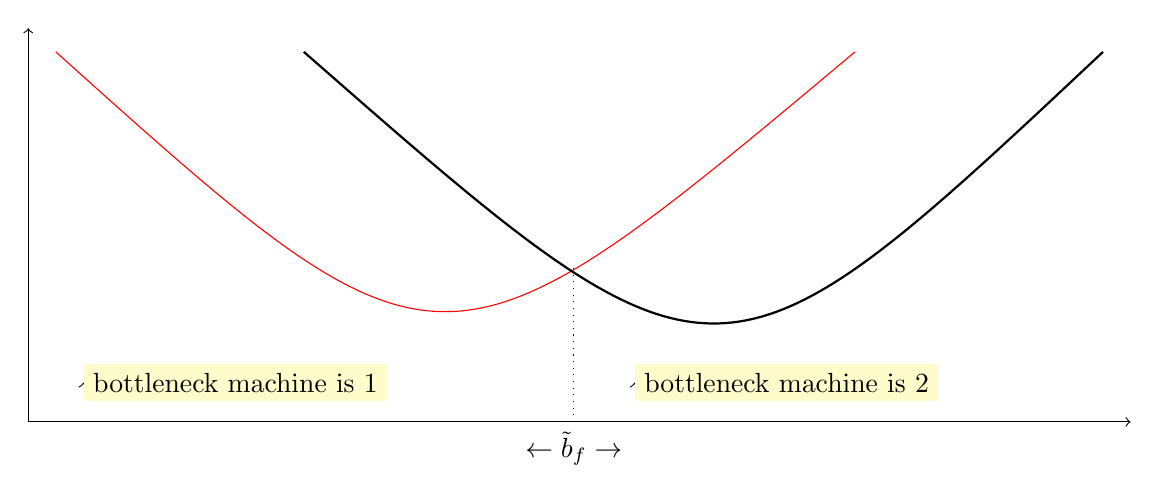
\begin{tikzpicture}[xscale=.7]
        \draw[<->] (0, 5) |- (20, 0);

        \draw[->] (1, .5) node[fill=yellow!20, right] {bottleneck machine is $1$};
        \draw[->] (11, .5) node[fill=yellow!20, right] {bottleneck machine is $2$};

        \draw[red] (0.5, 4.7) .. controls (7.5, .3) .. (15, 4.7);
        \draw[thick] (5, 4.7) .. controls (12.5, .1) .. (19.5, 4.7);
        \draw[dotted] (9.9, 0) node[below] {$\leftarrow\tilde b_f\rightarrow$} -- ++(0, 1.95);
    \end{tikzpicture}
    \caption{\label{produced_i:convex}Two different convex functions for finding "optimal" batch size}
\end{figure}

\subsubsection{Upper bound}

As previously said, computing the exact production time needed to produce $N$ items isn't an easy thing to do. However, a good upper bound for the production time, given a batch size $b_f$, can be computed as \[ T_{prod}(N)|_{b_f}\le T_{prod}(b_f) + \left( \left\lceil \frac{N}{b_f} \right\rceil - 1 \right)T_b(b_f) \] The error we're making in our estimate is then proportionnal to $\left\lceil \frac{N}{b_f} \right\rceil b_f - N$ where $\left\lceil \frac{N}{b_f} \right\rceil b_f$ represents the number of items for which we computed the production time and $N$ the aimed number of items. 

\subsection{Pull systems}

Concerning production systems which use the Kanban approach (also refered as pull systems), we can find a somehow analogous formula to compute an upper bound for the production time of $N$ items.

From the previous sections, we know that the ratio $D/D_i$ gives us the number of batches that machine $i$ delivers during a time window $D$. Thus, the working time of machine $i$ can be computed as \[ T_{wi} = \frac{D}{D_i}(T_{si}+T_{oi}b_i) \] Which equals, if we consider the batch sizing as $b_i = b_f n_{if}$, \[ \frac{D}{\frac{b_f}{X_f^{max}(b_f)}} (T_{si} + T_{oi}n_{if}) = D\frac{X_f^{max}(b_f)}{\frac{b_f}{T_{si}+T_{oi}n_{if}b_f}} \] since $D_i = D, \forall i$ and $D = b_f / X^{max}_f(b_f)$. Finally, noting that $X_f^{max} = \min\left( \frac{b_f}{T_{si} + T_{oi}b_fn_{if}} \right)$, we conclude that in any case : \[ T_{wi} \le D \] Thus, it stands that, since the time to produce the first batch is given by $L.D$ where $L$ is the level of the Bill of Material, an upper bound for the production time of $N$ items using batch sized as $b_i = b_fn_{if}$ in the pull production system is :
\[
    T_{prod}^{pull}(N)|_{b_f} = LD + \left\lceil \frac{N}{b_f} - 1 \right\rceil D
\]
This is very analogous to the previous formula obtained when dealing with push systems since here, the production cycle $D$ is determined by the bottleneck machine ($D = T_b(b_f)$). 

\subsection{Conclusion}

We end up with two estimates for an upper bound of the time to produce $N$ items which are : 
\[
    \begin{split}
        T_{prod}^{push}(N)|_{b_f} &\le T_{prod}(b_f) + \left( \left\lceil \frac{N}{b_f} \right\rceil - 1 \right)T_b(b_f)\\
        T_{prod}^{pull}(N)|_{b_f} &\le LD + \left( \left\lceil \frac{N}{b_f}\right\rceil - 1 \right) T_b(b_f)
    \end{split}
\]

And it can be easily seen that $T_{prod}^{push}(b_f) \le LD$ which imples the following relation between our two upper bounds : 
\[ T_{prod}^{push}(N)|_{b_f} \le T_{prod}^{pull}(N)|_{b_f} \]
But since our goal is to find a "reasonable" time to be considered for the production of $N$ items, for instance to tell our consumer that the production will be ready by that time and that he should come pick up our final products, one may always use the second formula even for \textit{push} systems since (1) it is an upper bound of the production time and (2) we end with a uniform formula. 

\subsection{Computing upper bounds : one final example}

\begin{wrapfigure}[14]{l}{4cm}
    \centering
    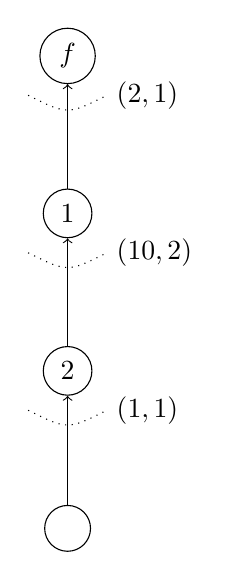
\begin{tikzpicture}
        \draw (0, 0) node[draw, circle] (f) {$f$};
        \draw (0, -2) node[draw, circle] (1) {$1$};
        \draw (0, -4) node[draw, circle] (2) {$2$};
        \draw (0, -6) node[draw, circle] (RM) {$\vphantom{j}$};

        \draw[dotted] (-.5, -.5) .. controls (0, -.75) .. (.5, -.5) node[right] {$(2, 1)$};
        \draw[dotted] (-.5, -2.5) .. controls (0, -2.75) .. (.5, -2.5) node[right] {$(10, 2)$};
        \draw[dotted] (-.5, -4.5) .. controls (0, -4.75) .. (.5, -4.5) node[right] {$(1, 1)$};

        \draw[<-] (f) -- (1);
        \draw[->] (2) -- (1);
        \draw[<-] (2) -- (RM);
    \end{tikzpicture}
    \caption{\label{produced_i:simple_bom}Example}
\end{wrapfigure}

Consider figure (\ref{produced_i:simple_bom}) which represents a very simple bill of material. Let's assume that one client orders $N = 70$ final products. When should we tell him to come back to pick up his goods ? We will do the computations studying various batch sizes among $10, 7$ and $6$. 

\subsubsection{Using push systems}

Using the previously established formula, we can compute an upper bound of the time needed to produce $N=70$ items like so :
\[
    T_{prod}^{push}(70)|_{b_f = 10} = (\underline{1 + 1.10} + \underline{ 10 + 2.10 } + \underline{ 2 + 1.10 } ) + (7-1)(10 + 2.10) = 233
\] since with $b_f = 10$, machine number $1$ is the bottleneck machine. Note that, in this situation, the computed upper bound is actually the "supremum" (the best upper bound we can found) which coincides with the exact value of $T_{prod}^{push}$ since $70$ is a multiple of $10$. 

Similar computations gives the following results : 
\[
    \begin{split}
        T_{prod}^{push}(70)|_{b_f = 7} &= 257\\
        T_{prod}^{push}(70)|_{b_f = 6} &\le 279\\
    \end{split}
\]
And note that, in the latter case, the result is an upper bound which differs from the exact value of the production time needed since $6$ is not a divisor of $70$. Actually, we are estimating our upper bound by computing the time needed to produce $6\times 12 = 72$ items instead of $70$ since $\lceil 70 / 6 \rceil = 12$. 

\subsubsection{Using pull systems}

Using the corresponding formula for the pull systems, we can compute upper bounds in the same way. (Note that the formula can be rewritten as $T_{prod}^{pull}(N)_{b_f} = \left( L-1+\left\lceil \frac{N}{b_f} \right\rceil \right) T_b(b_f)$ which is handier to compute by hand...). Doing so, we get the following results : 

\[
    \begin{split}
        T_{prod}^{pull}(70)|_{b_f = 10} &\le (3 - 1 + 7).30 = 270\\
        T_{prod}^{pull}(70)|_{b_f = 7} &\le 288\\
        T_{prod}^{pull}(70)|_{b_f = 6} &\le 308\\
    \end{split}
\]

Which gives as expected greater upper bounds but sufficiently good ones.

\subsubsection{Optimal batch sizing ?}

Just like we did in the section dedicated to push systems, and since we know that we can use one uniformed formula, let's suppose $N/b_f$ to be integer and let's assume knowing the bottleneck machine corresponding to the optimal batch size, our upper bound can be given by \[
    \begin{split}
        T_{prod}(N)_{b_f} &= \left(L - 1 \frac{N}{b_f}\right)T_b(b_f) \\
        &= \left(L-1\frac{N}{b_f}\right) ( T_{sb} + T_{ob}b_fn_{bf} ) \\
        &= \frac{N}{b_f}T_{sb} + (L-1)T_{ob}b_fn_{b_f} + (L-1)T_{sb} + NT_{ob}n_{bf}
    \end{split}
\]
And let's take the derivative of this function with respect to $b_f$, it yields 
\[
    \frac{dT_{prod}}{db_f} = -\frac{N}{b_f^2} + (L-1)T_{ob}b_fn_{bf}
\]
Which is convex and yields the optimal solution \[ b_f^\circ = \sqrt{ \frac{NT_{sb}}{ (L-1)T_{ob}n_{bf} } } \]
But keep in mind that, similarly to what have been said in the previous section, this formula holds only if the bottleneck machine was well the one we had supposed it would be. That is, we have to check \textit{a posteriori} that the bottleneck machine we considered for our computation is well the one corresponding to the batch size $b_f^\circ$. 

Looking back at our example, we obtain the "optimal" batch size (supposing that $1$ will be the bottleneck machine) as $b_f^\circ = \sqrt{ \frac{70.10}{2.2} } \approx 14$. Using such a batch size\footnote{which is relevant since the bottleneck machine associated to that batch size is well machine $1$} will result in the "smallest" production time estimate using the established formula which are \[
    \begin{split}
    T_{prod}^{push}(70)|_{b_f = 14} &= 221\\
    T_{prod}^{push}(70)|_{b_f = 14} &= 266\\
    \end{split}
    \]

\section{Arbitrary batch sizing}

Our final consideration concerning the computation of the time needed to produce a fixed number of items $N$ is the one related to the situation in which $b_i\ne b_fn_{if}$. We have seen that the only way of producing using an arbitrary batch size is to use the Kanban system. In this case, we are dealing with different batch sizes for each machine $b_i$ which are arbitrary choosen. We have already established that $\frac{D}{D_i}=K_i$ gives us the number of batches of product $i$ produced during the time window $D$. Thus, $K_ib_i$ returns the number of items $i$ produced during one production cycle $D$ and $\left\lceil \frac{N}{K_fb_f} \right\rceil$ equals the number of production cycle $D$ needed in order to produce $N$ items. Thus, the following formula holds:  
\[
    T_{prod}(N)|_{\underline b} = LD + \left(\left\lceil \frac{N}{K_fb_f} \right\rceil - 1\right)D
\]
Which is a generalization of the previous formula when $b_i = b_fn_{if}$ since in this case we have $K_f = 1$. 

\end{document}